\documentclass[twoside]{book}

% Packages required by doxygen
\usepackage{fixltx2e}
\usepackage{calc}
\usepackage{doxygen}
\usepackage[export]{adjustbox} % also loads graphicx
\usepackage{graphicx}
\usepackage[utf8]{inputenc}
\usepackage{makeidx}
\usepackage{multicol}
\usepackage{multirow}
\PassOptionsToPackage{warn}{textcomp}
\usepackage{textcomp}
\usepackage[nointegrals]{wasysym}
\usepackage[table]{xcolor}

% Font selection
\usepackage[T1]{fontenc}
\usepackage[scaled=.90]{helvet}
\usepackage{courier}
\usepackage{amssymb}
\usepackage{sectsty}
\renewcommand{\familydefault}{\sfdefault}
\allsectionsfont{%
  \fontseries{bc}\selectfont%
  \color{darkgray}%
}
\renewcommand{\DoxyLabelFont}{%
  \fontseries{bc}\selectfont%
  \color{darkgray}%
}
\newcommand{\+}{\discretionary{\mbox{\scriptsize$\hookleftarrow$}}{}{}}

% Page & text layout
\usepackage{geometry}
\geometry{%
  a4paper,%
  top=2.5cm,%
  bottom=2.5cm,%
  left=2.5cm,%
  right=2.5cm%
}
\tolerance=750
\hfuzz=15pt
\hbadness=750
\setlength{\emergencystretch}{15pt}
\setlength{\parindent}{0cm}
\setlength{\parskip}{3ex plus 2ex minus 2ex}
\makeatletter
\renewcommand{\paragraph}{%
  \@startsection{paragraph}{4}{0ex}{-1.0ex}{1.0ex}{%
    \normalfont\normalsize\bfseries\SS@parafont%
  }%
}
\renewcommand{\subparagraph}{%
  \@startsection{subparagraph}{5}{0ex}{-1.0ex}{1.0ex}{%
    \normalfont\normalsize\bfseries\SS@subparafont%
  }%
}
\makeatother

% Headers & footers
\usepackage{fancyhdr}
\pagestyle{fancyplain}
\fancyhead[LE]{\fancyplain{}{\bfseries\thepage}}
\fancyhead[CE]{\fancyplain{}{}}
\fancyhead[RE]{\fancyplain{}{\bfseries\leftmark}}
\fancyhead[LO]{\fancyplain{}{\bfseries\rightmark}}
\fancyhead[CO]{\fancyplain{}{}}
\fancyhead[RO]{\fancyplain{}{\bfseries\thepage}}
\fancyfoot[LE]{\fancyplain{}{}}
\fancyfoot[CE]{\fancyplain{}{}}
\fancyfoot[RE]{\fancyplain{}{\bfseries\scriptsize Generated by Doxygen }}
\fancyfoot[LO]{\fancyplain{}{\bfseries\scriptsize Generated by Doxygen }}
\fancyfoot[CO]{\fancyplain{}{}}
\fancyfoot[RO]{\fancyplain{}{}}
\renewcommand{\footrulewidth}{0.4pt}
\renewcommand{\chaptermark}[1]{%
  \markboth{#1}{}%
}
\renewcommand{\sectionmark}[1]{%
  \markright{\thesection\ #1}%
}

% Indices & bibliography
\usepackage{natbib}
\usepackage[titles]{tocloft}
\setcounter{tocdepth}{3}
\setcounter{secnumdepth}{5}
\makeindex

% Hyperlinks (required, but should be loaded last)
\usepackage{ifpdf}
\ifpdf
  \usepackage[pdftex,pagebackref=true]{hyperref}
\else
  \usepackage[ps2pdf,pagebackref=true]{hyperref}
\fi
\hypersetup{%
  colorlinks=true,%
  linkcolor=blue,%
  citecolor=blue,%
  unicode%
}

% Custom commands
\newcommand{\clearemptydoublepage}{%
  \newpage{\pagestyle{empty}\cleardoublepage}%
}

\usepackage{caption}
\captionsetup{labelsep=space,justification=centering,font={bf},singlelinecheck=off,skip=4pt,position=top}

%===== C O N T E N T S =====

\begin{document}

% Titlepage & ToC
\hypersetup{pageanchor=false,
             bookmarksnumbered=true,
             pdfencoding=unicode
            }
\pagenumbering{alph}
\begin{titlepage}
\vspace*{7cm}
\begin{center}%
{\Large A\+S\+E6030 }\\
\vspace*{1cm}
{\large Generated by Doxygen 1.8.13}\\
\end{center}
\end{titlepage}
\clearemptydoublepage
\pagenumbering{roman}
\tableofcontents
\clearemptydoublepage
\pagenumbering{arabic}
\hypersetup{pageanchor=true}

%--- Begin generated contents ---
\chapter{A\+S\+E6030}
\label{md__r_e_a_d_m_e}
\Hypertarget{md__r_e_a_d_m_e}
A control system project 
\chapter{Namespace Index}
\section{Namespace List}
Here is a list of all documented namespaces with brief descriptions\+:\begin{DoxyCompactList}
\item\contentsline{section}{\hyperlink{namespace_a_s_e6030}{A\+S\+E6030} \\*A school project }{\pageref{namespace_a_s_e6030}}{}
\item\contentsline{section}{\hyperlink{namespace_a_s_e6030_1_1_properties}{A\+S\+E6030.\+Properties} }{\pageref{namespace_a_s_e6030_1_1_properties}}{}
\item\contentsline{section}{\hyperlink{namespace_controller_unit_test}{Controller\+Unit\+Test} }{\pageref{namespace_controller_unit_test}}{}
\end{DoxyCompactList}

\chapter{Hierarchical Index}
\section{Class Hierarchy}
This inheritance list is sorted roughly, but not completely, alphabetically\+:\begin{DoxyCompactList}
\item Application\begin{DoxyCompactList}
\item \contentsline{section}{A\+S\+E6030.\+App}{\pageref{class_a_s_e6030_1_1_app}}{}
\item \contentsline{section}{A\+S\+E6030.\+App}{\pageref{class_a_s_e6030_1_1_app}}{}
\item \contentsline{section}{A\+S\+E6030.\+App}{\pageref{class_a_s_e6030_1_1_app}}{}
\item \contentsline{section}{A\+S\+E6030.\+App}{\pageref{class_a_s_e6030_1_1_app}}{}
\end{DoxyCompactList}
\item \contentsline{section}{A\+S\+E6030.\+Controller}{\pageref{class_a_s_e6030_1_1_controller}}{}
\item \contentsline{section}{A\+S\+E6030.\+Flow\+Control\+Valve}{\pageref{class_a_s_e6030_1_1_flow_control_valve}}{}
\item \contentsline{section}{A\+S\+E6030.\+Heater}{\pageref{class_a_s_e6030_1_1_heater}}{}
\item I\+Component\+Connector\begin{DoxyCompactList}
\item \contentsline{section}{A\+S\+E6030.\+Main\+Window}{\pageref{class_a_s_e6030_1_1_main_window}}{}
\item \contentsline{section}{A\+S\+E6030.\+Main\+Window}{\pageref{class_a_s_e6030_1_1_main_window}}{}
\item \contentsline{section}{A\+S\+E6030.\+Main\+Window}{\pageref{class_a_s_e6030_1_1_main_window}}{}
\end{DoxyCompactList}
\item \contentsline{section}{A\+S\+E6030.\+Listener}{\pageref{class_a_s_e6030_1_1_listener}}{}
\item \contentsline{section}{A\+S\+E6030.\+On\+Off\+Valve}{\pageref{class_a_s_e6030_1_1_on_off_valve}}{}
\item \contentsline{section}{A\+S\+E6030.\+Pump}{\pageref{class_a_s_e6030_1_1_pump}}{}
\item \contentsline{section}{A\+S\+E6030.\+Sequence\+Parameters}{\pageref{class_a_s_e6030_1_1_sequence_parameters}}{}
\item \contentsline{section}{Controller\+Unit\+Test.\+Unit\+Test1}{\pageref{class_controller_unit_test_1_1_unit_test1}}{}
\item Window\begin{DoxyCompactList}
\item \contentsline{section}{A\+S\+E6030.\+Main\+Window}{\pageref{class_a_s_e6030_1_1_main_window}}{}
\item \contentsline{section}{A\+S\+E6030.\+Main\+Window}{\pageref{class_a_s_e6030_1_1_main_window}}{}
\item \contentsline{section}{A\+S\+E6030.\+Main\+Window}{\pageref{class_a_s_e6030_1_1_main_window}}{}
\item \contentsline{section}{A\+S\+E6030.\+Main\+Window}{\pageref{class_a_s_e6030_1_1_main_window}}{}
\end{DoxyCompactList}
\end{DoxyCompactList}

\chapter{Class Index}
\section{Class List}
Here are the classes, structs, unions and interfaces with brief descriptions\+:\begin{DoxyCompactList}
\item\contentsline{section}{\hyperlink{class_a_s_e6030_1_1_app}{A\+S\+E6030.\+App} \\*Interaction logic for App.\+xaml }{\pageref{class_a_s_e6030_1_1_app}}{}
\item\contentsline{section}{\hyperlink{class_a_s_e6030_1_1_controller}{A\+S\+E6030.\+Controller} \\*The controller logic }{\pageref{class_a_s_e6030_1_1_controller}}{}
\item\contentsline{section}{\hyperlink{class_a_s_e6030_1_1_flow_control_valve}{A\+S\+E6030.\+Flow\+Control\+Valve} \\*Class for controlling a flow control valve }{\pageref{class_a_s_e6030_1_1_flow_control_valve}}{}
\item\contentsline{section}{\hyperlink{class_a_s_e6030_1_1_heater}{A\+S\+E6030.\+Heater} \\*Class for controlling on/off heater element }{\pageref{class_a_s_e6030_1_1_heater}}{}
\item\contentsline{section}{\hyperlink{class_a_s_e6030_1_1_listener}{A\+S\+E6030.\+Listener} \\*Class listening for changes in the system }{\pageref{class_a_s_e6030_1_1_listener}}{}
\item\contentsline{section}{\hyperlink{class_a_s_e6030_1_1_main_window}{A\+S\+E6030.\+Main\+Window} \\*Interaction logic for Main\+Window.\+xaml }{\pageref{class_a_s_e6030_1_1_main_window}}{}
\item\contentsline{section}{\hyperlink{class_a_s_e6030_1_1_on_off_valve}{A\+S\+E6030.\+On\+Off\+Valve} \\*Class for controlling an On/\+Off valve }{\pageref{class_a_s_e6030_1_1_on_off_valve}}{}
\item\contentsline{section}{\hyperlink{class_a_s_e6030_1_1_pump}{A\+S\+E6030.\+Pump} \\*Class for controlling a pump }{\pageref{class_a_s_e6030_1_1_pump}}{}
\item\contentsline{section}{\hyperlink{class_a_s_e6030_1_1_sequence_parameters}{A\+S\+E6030.\+Sequence\+Parameters} \\*Class for saving the sequence parameters from user }{\pageref{class_a_s_e6030_1_1_sequence_parameters}}{}
\item\contentsline{section}{\hyperlink{class_controller_unit_test_1_1_unit_test1}{Controller\+Unit\+Test.\+Unit\+Test1} \\*Unit test for Controller class }{\pageref{class_controller_unit_test_1_1_unit_test1}}{}
\end{DoxyCompactList}

\chapter{Namespace Documentation}
\hypertarget{namespace_a_s_e6030}{}\section{A\+S\+E6030 Namespace Reference}
\label{namespace_a_s_e6030}\index{A\+S\+E6030@{A\+S\+E6030}}
\subsection*{Namespaces}
\begin{DoxyCompactItemize}
\end{DoxyCompactItemize}
\subsection*{Classes}
\begin{DoxyCompactItemize}
\item 
class \hyperlink{class_a_s_e6030_1_1_app}{App}
\begin{DoxyCompactList}\small\item\em Interaction logic for App.\+xaml \end{DoxyCompactList}\item 
class \hyperlink{class_a_s_e6030_1_1_controller}{Controller}
\item 
class \hyperlink{class_a_s_e6030_1_1_flow_control_valve}{Flow\+Control\+Valve}
\item 
class \hyperlink{class_a_s_e6030_1_1_heater}{Heater}
\item 
class \hyperlink{class_a_s_e6030_1_1_listener}{Listener}
\item 
class \hyperlink{class_a_s_e6030_1_1_main_window}{Main\+Window}
\begin{DoxyCompactList}\small\item\em Interaction logic for Main\+Window.\+xaml \end{DoxyCompactList}\item 
class \hyperlink{class_a_s_e6030_1_1_on_off_valve}{On\+Off\+Valve}
\item 
class \hyperlink{class_a_s_e6030_1_1_pump}{Pump}
\item 
class \hyperlink{class_a_s_e6030_1_1_sequence_parameters}{Sequence\+Parameters}
\end{DoxyCompactItemize}

\hypertarget{namespace_a_s_e6030_1_1_properties}{}\section{A\+S\+E6030.\+Properties Namespace Reference}
\label{namespace_a_s_e6030_1_1_properties}\index{A\+S\+E6030.\+Properties@{A\+S\+E6030.\+Properties}}
\subsection*{Classes}
\begin{DoxyCompactItemize}
\item 
class {\bfseries Resources}
\begin{DoxyCompactList}\small\item\em A strongly-\/typed resource class, for looking up localized strings, etc. \end{DoxyCompactList}\item 
class {\bfseries Settings}
\end{DoxyCompactItemize}

\hypertarget{namespace_controller_unit_test}{}\section{Controller\+Unit\+Test Namespace Reference}
\label{namespace_controller_unit_test}\index{Controller\+Unit\+Test@{Controller\+Unit\+Test}}
\subsection*{Classes}
\begin{DoxyCompactItemize}
\item 
class \hyperlink{class_controller_unit_test_1_1_unit_test1}{Unit\+Test1}
\begin{DoxyCompactList}\small\item\em Unit test for Controller class \end{DoxyCompactList}\end{DoxyCompactItemize}

\chapter{Class Documentation}
\hypertarget{class_a_s_e6030_1_1_app}{}\section{A\+S\+E6030.\+App Class Reference}
\label{class_a_s_e6030_1_1_app}\index{A\+S\+E6030.\+App@{A\+S\+E6030.\+App}}


Interaction logic for App.\+xaml  


Inheritance diagram for A\+S\+E6030.\+App\+:\begin{figure}[H]
\begin{center}
\leavevmode
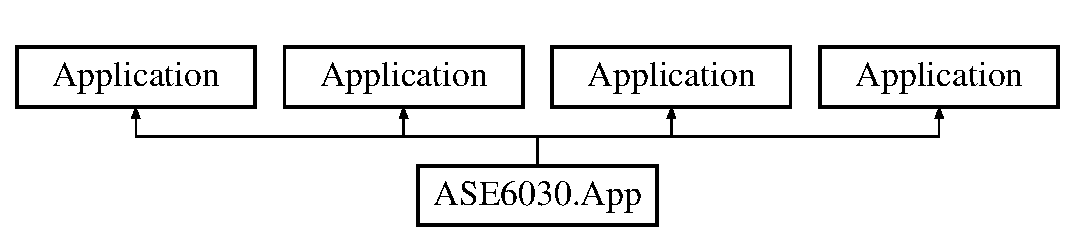
\includegraphics[height=2.000000cm]{class_a_s_e6030_1_1_app}
\end{center}
\end{figure}
\subsection*{Public Member Functions}
\begin{DoxyCompactItemize}
\item 
void \hyperlink{class_a_s_e6030_1_1_app_a3e92cf5b5ce00ab4725d8b49d4f4608b}{Initialize\+Component} ()
\begin{DoxyCompactList}\small\item\em Initialize\+Component \end{DoxyCompactList}\item 
void \hyperlink{class_a_s_e6030_1_1_app_a3e92cf5b5ce00ab4725d8b49d4f4608b}{Initialize\+Component} ()
\begin{DoxyCompactList}\small\item\em Initialize\+Component \end{DoxyCompactList}\item 
void \hyperlink{class_a_s_e6030_1_1_app_a3e92cf5b5ce00ab4725d8b49d4f4608b}{Initialize\+Component} ()
\begin{DoxyCompactList}\small\item\em Initialize\+Component \end{DoxyCompactList}\end{DoxyCompactItemize}
\subsection*{Static Public Member Functions}
\begin{DoxyCompactItemize}
\item 
static void \hyperlink{class_a_s_e6030_1_1_app_abf70d608fded53409f9aff64e8a723b3}{Main} ()
\begin{DoxyCompactList}\small\item\em Application Entry Point. \end{DoxyCompactList}\item 
static void \hyperlink{class_a_s_e6030_1_1_app_abf70d608fded53409f9aff64e8a723b3}{Main} ()
\begin{DoxyCompactList}\small\item\em Application Entry Point. \end{DoxyCompactList}\item 
static void \hyperlink{class_a_s_e6030_1_1_app_abf70d608fded53409f9aff64e8a723b3}{Main} ()
\begin{DoxyCompactList}\small\item\em Application Entry Point. \end{DoxyCompactList}\end{DoxyCompactItemize}


\subsection{Detailed Description}
Interaction logic for App.\+xaml 

\hyperlink{class_a_s_e6030_1_1_app}{App} 

\subsection{Member Function Documentation}
\mbox{\Hypertarget{class_a_s_e6030_1_1_app_a3e92cf5b5ce00ab4725d8b49d4f4608b}\label{class_a_s_e6030_1_1_app_a3e92cf5b5ce00ab4725d8b49d4f4608b}} 
\index{A\+S\+E6030\+::\+App@{A\+S\+E6030\+::\+App}!Initialize\+Component@{Initialize\+Component}}
\index{Initialize\+Component@{Initialize\+Component}!A\+S\+E6030\+::\+App@{A\+S\+E6030\+::\+App}}
\subsubsection{\texorpdfstring{Initialize\+Component()}{InitializeComponent()}\hspace{0.1cm}{\footnotesize\ttfamily [1/3]}}
{\footnotesize\ttfamily void A\+S\+E6030.\+App.\+Initialize\+Component (\begin{DoxyParamCaption}{ }\end{DoxyParamCaption})\hspace{0.3cm}{\ttfamily [inline]}}



Initialize\+Component 

\mbox{\Hypertarget{class_a_s_e6030_1_1_app_a3e92cf5b5ce00ab4725d8b49d4f4608b}\label{class_a_s_e6030_1_1_app_a3e92cf5b5ce00ab4725d8b49d4f4608b}} 
\index{A\+S\+E6030\+::\+App@{A\+S\+E6030\+::\+App}!Initialize\+Component@{Initialize\+Component}}
\index{Initialize\+Component@{Initialize\+Component}!A\+S\+E6030\+::\+App@{A\+S\+E6030\+::\+App}}
\subsubsection{\texorpdfstring{Initialize\+Component()}{InitializeComponent()}\hspace{0.1cm}{\footnotesize\ttfamily [2/3]}}
{\footnotesize\ttfamily void A\+S\+E6030.\+App.\+Initialize\+Component (\begin{DoxyParamCaption}{ }\end{DoxyParamCaption})\hspace{0.3cm}{\ttfamily [inline]}}



Initialize\+Component 

\mbox{\Hypertarget{class_a_s_e6030_1_1_app_a3e92cf5b5ce00ab4725d8b49d4f4608b}\label{class_a_s_e6030_1_1_app_a3e92cf5b5ce00ab4725d8b49d4f4608b}} 
\index{A\+S\+E6030\+::\+App@{A\+S\+E6030\+::\+App}!Initialize\+Component@{Initialize\+Component}}
\index{Initialize\+Component@{Initialize\+Component}!A\+S\+E6030\+::\+App@{A\+S\+E6030\+::\+App}}
\subsubsection{\texorpdfstring{Initialize\+Component()}{InitializeComponent()}\hspace{0.1cm}{\footnotesize\ttfamily [3/3]}}
{\footnotesize\ttfamily void A\+S\+E6030.\+App.\+Initialize\+Component (\begin{DoxyParamCaption}{ }\end{DoxyParamCaption})\hspace{0.3cm}{\ttfamily [inline]}}



Initialize\+Component 

\mbox{\Hypertarget{class_a_s_e6030_1_1_app_abf70d608fded53409f9aff64e8a723b3}\label{class_a_s_e6030_1_1_app_abf70d608fded53409f9aff64e8a723b3}} 
\index{A\+S\+E6030\+::\+App@{A\+S\+E6030\+::\+App}!Main@{Main}}
\index{Main@{Main}!A\+S\+E6030\+::\+App@{A\+S\+E6030\+::\+App}}
\subsubsection{\texorpdfstring{Main()}{Main()}\hspace{0.1cm}{\footnotesize\ttfamily [1/3]}}
{\footnotesize\ttfamily static void A\+S\+E6030.\+App.\+Main (\begin{DoxyParamCaption}{ }\end{DoxyParamCaption})\hspace{0.3cm}{\ttfamily [inline]}, {\ttfamily [static]}}



Application Entry Point. 

\mbox{\Hypertarget{class_a_s_e6030_1_1_app_abf70d608fded53409f9aff64e8a723b3}\label{class_a_s_e6030_1_1_app_abf70d608fded53409f9aff64e8a723b3}} 
\index{A\+S\+E6030\+::\+App@{A\+S\+E6030\+::\+App}!Main@{Main}}
\index{Main@{Main}!A\+S\+E6030\+::\+App@{A\+S\+E6030\+::\+App}}
\subsubsection{\texorpdfstring{Main()}{Main()}\hspace{0.1cm}{\footnotesize\ttfamily [2/3]}}
{\footnotesize\ttfamily static void A\+S\+E6030.\+App.\+Main (\begin{DoxyParamCaption}{ }\end{DoxyParamCaption})\hspace{0.3cm}{\ttfamily [inline]}, {\ttfamily [static]}}



Application Entry Point. 

\mbox{\Hypertarget{class_a_s_e6030_1_1_app_abf70d608fded53409f9aff64e8a723b3}\label{class_a_s_e6030_1_1_app_abf70d608fded53409f9aff64e8a723b3}} 
\index{A\+S\+E6030\+::\+App@{A\+S\+E6030\+::\+App}!Main@{Main}}
\index{Main@{Main}!A\+S\+E6030\+::\+App@{A\+S\+E6030\+::\+App}}
\subsubsection{\texorpdfstring{Main()}{Main()}\hspace{0.1cm}{\footnotesize\ttfamily [3/3]}}
{\footnotesize\ttfamily static void A\+S\+E6030.\+App.\+Main (\begin{DoxyParamCaption}{ }\end{DoxyParamCaption})\hspace{0.3cm}{\ttfamily [inline]}, {\ttfamily [static]}}



Application Entry Point. 



The documentation for this class was generated from the following files\+:\begin{DoxyCompactItemize}
\item 
A\+S\+E6030/App.\+xaml.\+cs\item 
A\+S\+E6030/obj/x86/\+Debug/App.\+g.\+cs\item 
A\+S\+E6030/obj/x86/\+Debug/App.\+g.\+i.\+cs\end{DoxyCompactItemize}

\hypertarget{class_a_s_e6030_1_1_controller}{}\section{A\+S\+E6030.\+Controller Class Reference}
\label{class_a_s_e6030_1_1_controller}\index{A\+S\+E6030.\+Controller@{A\+S\+E6030.\+Controller}}


The controller logic  


\subsection*{Public Member Functions}
\begin{DoxyCompactItemize}
\item 
\hyperlink{class_a_s_e6030_1_1_controller_aa7df468c34d983c6efe88f12abeffb79}{Controller} (\hyperlink{class_a_s_e6030_1_1_main_window}{Main\+Window} window)
\begin{DoxyCompactList}\small\item\em Constructor. \end{DoxyCompactList}\item 
void \hyperlink{class_a_s_e6030_1_1_controller_a5f84e69b4885c561df4bc177fcc54d40}{connect\+Client} (string U\+RL)
\begin{DoxyCompactList}\small\item\em Connect to selected client. \end{DoxyCompactList}\item 
\mbox{\Hypertarget{class_a_s_e6030_1_1_controller_add4e6755696e2d0525bbb9fb8a5c8155}\label{class_a_s_e6030_1_1_controller_add4e6755696e2d0525bbb9fb8a5c8155}} 
string \hyperlink{class_a_s_e6030_1_1_controller_add4e6755696e2d0525bbb9fb8a5c8155}{get\+U\+RL} ()
\begin{DoxyCompactList}\small\item\em Returns the current U\+RL for device to be connected. Mainly for testing purposes. \end{DoxyCompactList}\item 
void \hyperlink{class_a_s_e6030_1_1_controller_afee09ba01da47aa772ce3da642e08e47}{set\+Params} (\hyperlink{class_a_s_e6030_1_1_sequence_parameters}{Sequence\+Parameters} parameters)
\item 
void \hyperlink{class_a_s_e6030_1_1_controller_afca76c3628ed37f21c1aac044a5e0441}{start\+Sequence} ()
\begin{DoxyCompactList}\small\item\em Start the sequence. \end{DoxyCompactList}\item 
void \hyperlink{class_a_s_e6030_1_1_controller_a1fa113ab02226c2d8a678365a749e3b0}{abort\+Sequence} ()
\begin{DoxyCompactList}\small\item\em Abort sequence. \end{DoxyCompactList}\end{DoxyCompactItemize}
\subsection*{Public Attributes}
\begin{DoxyCompactItemize}
\item 
\mbox{\Hypertarget{class_a_s_e6030_1_1_controller_a36785106c3f4bc54402290b0d86911fc}\label{class_a_s_e6030_1_1_controller_a36785106c3f4bc54402290b0d86911fc}} 
Tut.\+Mpp\+Opc\+Ua\+Client\+Lib.\+Mpp\+Client {\bfseries client}
\item 
\mbox{\Hypertarget{class_a_s_e6030_1_1_controller_a8cc31711b16a81099afb9ad6125d1d0f}\label{class_a_s_e6030_1_1_controller_a8cc31711b16a81099afb9ad6125d1d0f}} 
\hyperlink{class_a_s_e6030_1_1_listener}{Listener} {\bfseries listener}
\end{DoxyCompactItemize}
\subsection*{Private Member Functions}
\begin{DoxyCompactItemize}
\item 
void \hyperlink{class_a_s_e6030_1_1_controller_ac13cb64488eb479527e08d4af8f29869}{start\+Listener} ()
\item 
\mbox{\Hypertarget{class_a_s_e6030_1_1_controller_a1a0e5a9d392358ae55514c201631591c}\label{class_a_s_e6030_1_1_controller_a1a0e5a9d392358ae55514c201631591c}} 
void \hyperlink{class_a_s_e6030_1_1_controller_a1a0e5a9d392358ae55514c201631591c}{assign\+Units} ()
\begin{DoxyCompactList}\small\item\em Create objects for all units to be controlled. \end{DoxyCompactList}\item 
\mbox{\Hypertarget{class_a_s_e6030_1_1_controller_aaad2a679e6a2f5db4193f58fd7482def}\label{class_a_s_e6030_1_1_controller_aaad2a679e6a2f5db4193f58fd7482def}} 
void \hyperlink{class_a_s_e6030_1_1_controller_aaad2a679e6a2f5db4193f58fd7482def}{start\+Impregnation} ()
\begin{DoxyCompactList}\small\item\em Start Impregnation step in its own thread, followed by Black Liquor Fill. \end{DoxyCompactList}\item 
\mbox{\Hypertarget{class_a_s_e6030_1_1_controller_ac60700638fa6ac183134d3e9b6aa1005}\label{class_a_s_e6030_1_1_controller_ac60700638fa6ac183134d3e9b6aa1005}} 
void \hyperlink{class_a_s_e6030_1_1_controller_ac60700638fa6ac183134d3e9b6aa1005}{start\+Black\+Liquor\+Fill} ()
\begin{DoxyCompactList}\small\item\em Start Black Liquor Fill step in its own thread, followed by White Liquor Fill. \end{DoxyCompactList}\item 
\mbox{\Hypertarget{class_a_s_e6030_1_1_controller_a4e3027f9fd319e634cc11b9b9cc680c4}\label{class_a_s_e6030_1_1_controller_a4e3027f9fd319e634cc11b9b9cc680c4}} 
void \hyperlink{class_a_s_e6030_1_1_controller_a4e3027f9fd319e634cc11b9b9cc680c4}{start\+White\+Liquor\+Fill} ()
\begin{DoxyCompactList}\small\item\em Start White Liquor Fill step in its own thread, followed by Cooking. \end{DoxyCompactList}\item 
\mbox{\Hypertarget{class_a_s_e6030_1_1_controller_a0bc176e3b374f78d4d1ba4dd7d6542b6}\label{class_a_s_e6030_1_1_controller_a0bc176e3b374f78d4d1ba4dd7d6542b6}} 
void \hyperlink{class_a_s_e6030_1_1_controller_a0bc176e3b374f78d4d1ba4dd7d6542b6}{start\+Cooking} ()
\begin{DoxyCompactList}\small\item\em Start Cooking step in its own thread, followed by Discharge. \end{DoxyCompactList}\item 
\mbox{\Hypertarget{class_a_s_e6030_1_1_controller_aa881bbc599467936dbffc03ba2038906}\label{class_a_s_e6030_1_1_controller_aa881bbc599467936dbffc03ba2038906}} 
void \hyperlink{class_a_s_e6030_1_1_controller_aa881bbc599467936dbffc03ba2038906}{discharge} ()
\begin{DoxyCompactList}\small\item\em Start Discharge step in its own thread. \end{DoxyCompactList}\item 
void \hyperlink{class_a_s_e6030_1_1_controller_a9ce11137966555bf33690347e1e56cf7}{shut\+Down} ()
\begin{DoxyCompactList}\small\item\em Shut down all pumps, heater, close all valves. \end{DoxyCompactList}\item 
\mbox{\Hypertarget{class_a_s_e6030_1_1_controller_a2307744a7146425be174ec8acbe80e68}\label{class_a_s_e6030_1_1_controller_a2307744a7146425be174ec8acbe80e68}} 
void \hyperlink{class_a_s_e6030_1_1_controller_a2307744a7146425be174ec8acbe80e68}{E\+M1\+\_\+\+O\+P1} ()
\begin{DoxyCompactList}\small\item\em Open route to digester/\+T300, pump and heat. \end{DoxyCompactList}\item 
\mbox{\Hypertarget{class_a_s_e6030_1_1_controller_a136dfb3ec3897fbec64840958f841b46}\label{class_a_s_e6030_1_1_controller_a136dfb3ec3897fbec64840958f841b46}} 
void \hyperlink{class_a_s_e6030_1_1_controller_a136dfb3ec3897fbec64840958f841b46}{E\+M1\+\_\+\+O\+P2} ()
\begin{DoxyCompactList}\small\item\em Open route to digester/\+T300 and pump. \end{DoxyCompactList}\item 
\mbox{\Hypertarget{class_a_s_e6030_1_1_controller_ada67e644ad325022d583ccb45c8bc979}\label{class_a_s_e6030_1_1_controller_ada67e644ad325022d583ccb45c8bc979}} 
void \hyperlink{class_a_s_e6030_1_1_controller_ada67e644ad325022d583ccb45c8bc979}{E\+M1\+\_\+\+O\+P3} ()
\begin{DoxyCompactList}\small\item\em Close route to digester/\+T300, pump and heater off. \end{DoxyCompactList}\item 
\mbox{\Hypertarget{class_a_s_e6030_1_1_controller_a1a77c72e15f8e4341864266e1c883dc8}\label{class_a_s_e6030_1_1_controller_a1a77c72e15f8e4341864266e1c883dc8}} 
void \hyperlink{class_a_s_e6030_1_1_controller_a1a77c72e15f8e4341864266e1c883dc8}{E\+M1\+\_\+\+O\+P4} ()
\begin{DoxyCompactList}\small\item\em Close route to digester/\+T300 and pump off. \end{DoxyCompactList}\item 
\mbox{\Hypertarget{class_a_s_e6030_1_1_controller_a3ee9ee83a0799f1c45edd53914b22f27}\label{class_a_s_e6030_1_1_controller_a3ee9ee83a0799f1c45edd53914b22f27}} 
void \hyperlink{class_a_s_e6030_1_1_controller_a3ee9ee83a0799f1c45edd53914b22f27}{E\+M2\+\_\+\+O\+P1} ()
\begin{DoxyCompactList}\small\item\em Look up the rest in tech details docs. \end{DoxyCompactList}\item 
\mbox{\Hypertarget{class_a_s_e6030_1_1_controller_a9f8e1bba080881b98fdd0d928316cfe9}\label{class_a_s_e6030_1_1_controller_a9f8e1bba080881b98fdd0d928316cfe9}} 
void {\bfseries E\+M2\+\_\+\+O\+P2} ()
\item 
\mbox{\Hypertarget{class_a_s_e6030_1_1_controller_a1f6f13495bcc83ae3bf46de1b1310a9b}\label{class_a_s_e6030_1_1_controller_a1f6f13495bcc83ae3bf46de1b1310a9b}} 
void {\bfseries E\+M3\+\_\+\+O\+P1} ()
\item 
\mbox{\Hypertarget{class_a_s_e6030_1_1_controller_a64848ea464607f95e91b1da92adc1aeb}\label{class_a_s_e6030_1_1_controller_a64848ea464607f95e91b1da92adc1aeb}} 
void {\bfseries E\+M3\+\_\+\+O\+P2} ()
\item 
\mbox{\Hypertarget{class_a_s_e6030_1_1_controller_a92b515c30c2599a8bf3e796bba73b9ce}\label{class_a_s_e6030_1_1_controller_a92b515c30c2599a8bf3e796bba73b9ce}} 
void {\bfseries E\+M3\+\_\+\+O\+P3} ()
\item 
\mbox{\Hypertarget{class_a_s_e6030_1_1_controller_a1a58465612fe09ca1edd010f462f156c}\label{class_a_s_e6030_1_1_controller_a1a58465612fe09ca1edd010f462f156c}} 
void {\bfseries E\+M3\+\_\+\+O\+P4} ()
\item 
\mbox{\Hypertarget{class_a_s_e6030_1_1_controller_a36821d2fcf2823a14d968d76c7746f56}\label{class_a_s_e6030_1_1_controller_a36821d2fcf2823a14d968d76c7746f56}} 
void {\bfseries E\+M3\+\_\+\+O\+P5} ()
\item 
\mbox{\Hypertarget{class_a_s_e6030_1_1_controller_a2375462bbd5c285383a163bcdc863cb1}\label{class_a_s_e6030_1_1_controller_a2375462bbd5c285383a163bcdc863cb1}} 
void {\bfseries E\+M3\+\_\+\+O\+P6} ()
\item 
\mbox{\Hypertarget{class_a_s_e6030_1_1_controller_a876559042576cdad5b618af7c0027e3f}\label{class_a_s_e6030_1_1_controller_a876559042576cdad5b618af7c0027e3f}} 
void {\bfseries E\+M3\+\_\+\+O\+P7} ()
\item 
\mbox{\Hypertarget{class_a_s_e6030_1_1_controller_a3e7140dbb56a32c9eb13c4b194042901}\label{class_a_s_e6030_1_1_controller_a3e7140dbb56a32c9eb13c4b194042901}} 
void \hyperlink{class_a_s_e6030_1_1_controller_a3e7140dbb56a32c9eb13c4b194042901}{E\+M3\+\_\+\+O\+P8} (int delay)
\begin{DoxyCompactList}\small\item\em Open V204, wait for time delay, close V204. Int delay in ms. \end{DoxyCompactList}\item 
\mbox{\Hypertarget{class_a_s_e6030_1_1_controller_a6d62a17fc0600c10bfd805275efe8615}\label{class_a_s_e6030_1_1_controller_a6d62a17fc0600c10bfd805275efe8615}} 
void {\bfseries E\+M4\+\_\+\+O\+P1} ()
\item 
\mbox{\Hypertarget{class_a_s_e6030_1_1_controller_a7e83967562237044f564c5dab7020f0a}\label{class_a_s_e6030_1_1_controller_a7e83967562237044f564c5dab7020f0a}} 
void {\bfseries E\+M4\+\_\+\+O\+P2} ()
\item 
\mbox{\Hypertarget{class_a_s_e6030_1_1_controller_aac309fed5ac5a1e1b14c91f0bc74384a}\label{class_a_s_e6030_1_1_controller_aac309fed5ac5a1e1b14c91f0bc74384a}} 
void {\bfseries E\+M5\+\_\+\+O\+P1} ()
\item 
\mbox{\Hypertarget{class_a_s_e6030_1_1_controller_ac1e21b41f4b6fd90dec2d942f3370183}\label{class_a_s_e6030_1_1_controller_ac1e21b41f4b6fd90dec2d942f3370183}} 
void {\bfseries E\+M5\+\_\+\+O\+P2} ()
\item 
\mbox{\Hypertarget{class_a_s_e6030_1_1_controller_a3db5e3e582ab32c0e112f5d23c0e0e52}\label{class_a_s_e6030_1_1_controller_a3db5e3e582ab32c0e112f5d23c0e0e52}} 
void {\bfseries E\+M5\+\_\+\+O\+P3} ()
\item 
\mbox{\Hypertarget{class_a_s_e6030_1_1_controller_ae24a7fd26d6686a1d7e2d1637df01b3d}\label{class_a_s_e6030_1_1_controller_ae24a7fd26d6686a1d7e2d1637df01b3d}} 
void {\bfseries E\+M5\+\_\+\+O\+P4} ()
\item 
\mbox{\Hypertarget{class_a_s_e6030_1_1_controller_a04581a4009f6c2f43e6d00a9ffe0f31b}\label{class_a_s_e6030_1_1_controller_a04581a4009f6c2f43e6d00a9ffe0f31b}} 
void {\bfseries U1\+\_\+\+O\+P1} ()
\item 
\mbox{\Hypertarget{class_a_s_e6030_1_1_controller_a88c7d72a188abbee855fadfa2b20b9c1}\label{class_a_s_e6030_1_1_controller_a88c7d72a188abbee855fadfa2b20b9c1}} 
void {\bfseries U1\+\_\+\+O\+P2} ()
\item 
\mbox{\Hypertarget{class_a_s_e6030_1_1_controller_ade672c393adf276892b83f1975868052}\label{class_a_s_e6030_1_1_controller_ade672c393adf276892b83f1975868052}} 
void {\bfseries U1\+\_\+\+O\+P3} ()
\item 
\mbox{\Hypertarget{class_a_s_e6030_1_1_controller_ad39c8081f96086a56d87761aaa7ca4a1}\label{class_a_s_e6030_1_1_controller_ad39c8081f96086a56d87761aaa7ca4a1}} 
void {\bfseries U1\+\_\+\+O\+P4} ()
\item 
\mbox{\Hypertarget{class_a_s_e6030_1_1_controller_a2b138dfba719951a59f240ff60c80979}\label{class_a_s_e6030_1_1_controller_a2b138dfba719951a59f240ff60c80979}} 
void {\bfseries Err} (string e)
\end{DoxyCompactItemize}
\subsection*{Private Attributes}
\begin{DoxyCompactItemize}
\item 
\mbox{\Hypertarget{class_a_s_e6030_1_1_controller_a10e880717ab8856d38db3bf3cde053c9}\label{class_a_s_e6030_1_1_controller_a10e880717ab8856d38db3bf3cde053c9}} 
\hyperlink{class_a_s_e6030_1_1_main_window}{Main\+Window} {\bfseries window}
\item 
\mbox{\Hypertarget{class_a_s_e6030_1_1_controller_a2e009a3dfc8bdf97720f80c4b964ac14}\label{class_a_s_e6030_1_1_controller_a2e009a3dfc8bdf97720f80c4b964ac14}} 
Tut.\+Mpp\+Opc\+Ua\+Client\+Lib.\+Mpp\+Client.\+Mpp\+Client\+Ctor\+Params {\bfseries simulator\+Params}
\item 
const string \hyperlink{class_a_s_e6030_1_1_controller_a6fca165bf2388426d598f23ac8d9acd6}{S\+I\+M\+U\+L\+A\+T\+O\+R\+\_\+\+U\+RL} = \char`\"{}opc.\+tcp\+://127.\+0.\+0.\+1\+:8087\char`\"{}
\item 
const string \hyperlink{class_a_s_e6030_1_1_controller_a2011ff29fbc80180267d0aba04e903aa}{D\+E\+V\+I\+C\+E\+\_\+\+U\+RL} = \char`\"{}opc.\+tcp\+://192.\+168.\+137.\+101\char`\"{}
\item 
\mbox{\Hypertarget{class_a_s_e6030_1_1_controller_a89786f98405cbb27933eb00182d03c9a}\label{class_a_s_e6030_1_1_controller_a89786f98405cbb27933eb00182d03c9a}} 
string {\bfseries U\+RL}
\item 
\mbox{\Hypertarget{class_a_s_e6030_1_1_controller_a64624861c96c4570085f096079a2e317}\label{class_a_s_e6030_1_1_controller_a64624861c96c4570085f096079a2e317}} 
int {\bfseries L\+O\+O\+P\+\_\+\+T\+I\+ME} = 200
\item 
\mbox{\Hypertarget{class_a_s_e6030_1_1_controller_a5ab5f075cbe2e1882c444557c57f7602}\label{class_a_s_e6030_1_1_controller_a5ab5f075cbe2e1882c444557c57f7602}} 
\hyperlink{class_a_s_e6030_1_1_pump}{Pump} {\bfseries p100}
\item 
\mbox{\Hypertarget{class_a_s_e6030_1_1_controller_a1e39f7d76e8e53e0927fbdf667860450}\label{class_a_s_e6030_1_1_controller_a1e39f7d76e8e53e0927fbdf667860450}} 
\hyperlink{class_a_s_e6030_1_1_pump}{Pump} {\bfseries p200}
\item 
\mbox{\Hypertarget{class_a_s_e6030_1_1_controller_aaa206db707757508ca7d76fd0f3ef339}\label{class_a_s_e6030_1_1_controller_aaa206db707757508ca7d76fd0f3ef339}} 
\hyperlink{class_a_s_e6030_1_1_on_off_valve}{On\+Off\+Valve} {\bfseries v103}
\item 
\mbox{\Hypertarget{class_a_s_e6030_1_1_controller_a12546e753b7aaf735aae184e384523d8}\label{class_a_s_e6030_1_1_controller_a12546e753b7aaf735aae184e384523d8}} 
\hyperlink{class_a_s_e6030_1_1_on_off_valve}{On\+Off\+Valve} {\bfseries v201}
\item 
\mbox{\Hypertarget{class_a_s_e6030_1_1_controller_a4d55b3ae012a7f16456fc0a39a64fe35}\label{class_a_s_e6030_1_1_controller_a4d55b3ae012a7f16456fc0a39a64fe35}} 
\hyperlink{class_a_s_e6030_1_1_on_off_valve}{On\+Off\+Valve} {\bfseries v204}
\item 
\mbox{\Hypertarget{class_a_s_e6030_1_1_controller_a658e4e5c136ccfbb10551b07cb9092e8}\label{class_a_s_e6030_1_1_controller_a658e4e5c136ccfbb10551b07cb9092e8}} 
\hyperlink{class_a_s_e6030_1_1_on_off_valve}{On\+Off\+Valve} {\bfseries v301}
\item 
\mbox{\Hypertarget{class_a_s_e6030_1_1_controller_a5d87a2afa1aea2bff23bd01881b4e8f3}\label{class_a_s_e6030_1_1_controller_a5d87a2afa1aea2bff23bd01881b4e8f3}} 
\hyperlink{class_a_s_e6030_1_1_on_off_valve}{On\+Off\+Valve} {\bfseries v302}
\item 
\mbox{\Hypertarget{class_a_s_e6030_1_1_controller_ae6b8b0b43264264d893a8e1dd731359b}\label{class_a_s_e6030_1_1_controller_ae6b8b0b43264264d893a8e1dd731359b}} 
\hyperlink{class_a_s_e6030_1_1_on_off_valve}{On\+Off\+Valve} {\bfseries v303}
\item 
\mbox{\Hypertarget{class_a_s_e6030_1_1_controller_a151cf48626d9fb077bdde06c754fe8f5}\label{class_a_s_e6030_1_1_controller_a151cf48626d9fb077bdde06c754fe8f5}} 
\hyperlink{class_a_s_e6030_1_1_on_off_valve}{On\+Off\+Valve} {\bfseries v304}
\item 
\mbox{\Hypertarget{class_a_s_e6030_1_1_controller_a3c95dda39597388cd343165ba3b7074e}\label{class_a_s_e6030_1_1_controller_a3c95dda39597388cd343165ba3b7074e}} 
\hyperlink{class_a_s_e6030_1_1_on_off_valve}{On\+Off\+Valve} {\bfseries v401}
\item 
\mbox{\Hypertarget{class_a_s_e6030_1_1_controller_a1808e69cc26aee7ed1f80c7aeddeb88c}\label{class_a_s_e6030_1_1_controller_a1808e69cc26aee7ed1f80c7aeddeb88c}} 
\hyperlink{class_a_s_e6030_1_1_on_off_valve}{On\+Off\+Valve} {\bfseries v404}
\item 
\mbox{\Hypertarget{class_a_s_e6030_1_1_controller_ae2ae40c880ccc21c4ccd0d621144362d}\label{class_a_s_e6030_1_1_controller_ae2ae40c880ccc21c4ccd0d621144362d}} 
\hyperlink{class_a_s_e6030_1_1_flow_control_valve}{Flow\+Control\+Valve} {\bfseries v102}
\item 
\mbox{\Hypertarget{class_a_s_e6030_1_1_controller_a436ad6644fb7bb1e5d27b7373d6b9304}\label{class_a_s_e6030_1_1_controller_a436ad6644fb7bb1e5d27b7373d6b9304}} 
\hyperlink{class_a_s_e6030_1_1_flow_control_valve}{Flow\+Control\+Valve} {\bfseries v104}
\item 
\mbox{\Hypertarget{class_a_s_e6030_1_1_controller_ad83b0066e7b02129efe2f9d2f9b27631}\label{class_a_s_e6030_1_1_controller_ad83b0066e7b02129efe2f9d2f9b27631}} 
\hyperlink{class_a_s_e6030_1_1_heater}{Heater} {\bfseries e100}
\item 
\mbox{\Hypertarget{class_a_s_e6030_1_1_controller_ab37c0d55369f717ea4b162f2362475df}\label{class_a_s_e6030_1_1_controller_ab37c0d55369f717ea4b162f2362475df}} 
Thread {\bfseries Listener\+Thread}
\item 
\mbox{\Hypertarget{class_a_s_e6030_1_1_controller_a40180cabc4c4b7614623b448653cacb1}\label{class_a_s_e6030_1_1_controller_a40180cabc4c4b7614623b448653cacb1}} 
Thread {\bfseries Impregnation\+Thread}
\item 
\mbox{\Hypertarget{class_a_s_e6030_1_1_controller_a8a50aa5188fafd9109639053e41b1294}\label{class_a_s_e6030_1_1_controller_a8a50aa5188fafd9109639053e41b1294}} 
Thread {\bfseries Black\+Liquor\+Thread}
\item 
\mbox{\Hypertarget{class_a_s_e6030_1_1_controller_ac00c480ed840ab161db7b357a4b2f411}\label{class_a_s_e6030_1_1_controller_ac00c480ed840ab161db7b357a4b2f411}} 
Thread {\bfseries White\+Liquor\+Thread}
\item 
\mbox{\Hypertarget{class_a_s_e6030_1_1_controller_a8bcee80fe2923783d2e5713ad8141ed3}\label{class_a_s_e6030_1_1_controller_a8bcee80fe2923783d2e5713ad8141ed3}} 
Thread {\bfseries Cooking\+Thread}
\item 
\mbox{\Hypertarget{class_a_s_e6030_1_1_controller_aa239bb200cd8c58c5e0d014d6ca144b9}\label{class_a_s_e6030_1_1_controller_aa239bb200cd8c58c5e0d014d6ca144b9}} 
Thread {\bfseries Discharge\+Thread}
\item 
\mbox{\Hypertarget{class_a_s_e6030_1_1_controller_a580fc43de5878745efbb498cec865f1a}\label{class_a_s_e6030_1_1_controller_a580fc43de5878745efbb498cec865f1a}} 
\hyperlink{class_a_s_e6030_1_1_sequence_parameters}{Sequence\+Parameters} {\bfseries parameters}
\end{DoxyCompactItemize}


\subsection{Detailed Description}
The controller logic 

Uses Tut.\+Mpp\+Opc\+Ua\+Client\+Lib library to connect to the process 

\subsection{Constructor \& Destructor Documentation}
\mbox{\Hypertarget{class_a_s_e6030_1_1_controller_aa7df468c34d983c6efe88f12abeffb79}\label{class_a_s_e6030_1_1_controller_aa7df468c34d983c6efe88f12abeffb79}} 
\index{A\+S\+E6030\+::\+Controller@{A\+S\+E6030\+::\+Controller}!Controller@{Controller}}
\index{Controller@{Controller}!A\+S\+E6030\+::\+Controller@{A\+S\+E6030\+::\+Controller}}
\subsubsection{\texorpdfstring{Controller()}{Controller()}}
{\footnotesize\ttfamily A\+S\+E6030.\+Controller.\+Controller (\begin{DoxyParamCaption}\item[{\hyperlink{class_a_s_e6030_1_1_main_window}{Main\+Window}}]{window }\end{DoxyParamCaption})\hspace{0.3cm}{\ttfamily [inline]}}



Constructor. 

Takes the main window as a parameter. Window is used to send update calls for G\+UI 

\subsection{Member Function Documentation}
\mbox{\Hypertarget{class_a_s_e6030_1_1_controller_a1fa113ab02226c2d8a678365a749e3b0}\label{class_a_s_e6030_1_1_controller_a1fa113ab02226c2d8a678365a749e3b0}} 
\index{A\+S\+E6030\+::\+Controller@{A\+S\+E6030\+::\+Controller}!abort\+Sequence@{abort\+Sequence}}
\index{abort\+Sequence@{abort\+Sequence}!A\+S\+E6030\+::\+Controller@{A\+S\+E6030\+::\+Controller}}
\subsubsection{\texorpdfstring{abort\+Sequence()}{abortSequence()}}
{\footnotesize\ttfamily void A\+S\+E6030.\+Controller.\+abort\+Sequence (\begin{DoxyParamCaption}{ }\end{DoxyParamCaption})\hspace{0.3cm}{\ttfamily [inline]}}



Abort sequence. 

Abort the sequence, kill all working threads, shut all valves, pumps, and heater, notify the mainwindow. Will not affect the listener thread. \mbox{\Hypertarget{class_a_s_e6030_1_1_controller_a5f84e69b4885c561df4bc177fcc54d40}\label{class_a_s_e6030_1_1_controller_a5f84e69b4885c561df4bc177fcc54d40}} 
\index{A\+S\+E6030\+::\+Controller@{A\+S\+E6030\+::\+Controller}!connect\+Client@{connect\+Client}}
\index{connect\+Client@{connect\+Client}!A\+S\+E6030\+::\+Controller@{A\+S\+E6030\+::\+Controller}}
\subsubsection{\texorpdfstring{connect\+Client()}{connectClient()}}
{\footnotesize\ttfamily void A\+S\+E6030.\+Controller.\+connect\+Client (\begin{DoxyParamCaption}\item[{string}]{U\+RL }\end{DoxyParamCaption})\hspace{0.3cm}{\ttfamily [inline]}}



Connect to selected client. 

Parameter \char`\"{}\+U\+R\+L\char`\"{} must be either \char`\"{}\+D\+E\+V\+I\+C\+E\char`\"{} or \char`\"{}\+S\+I\+M\+U\+L\+A\+T\+O\+R\char`\"{}. No other inputs supported for now. Simulator and device U\+R\+Ls hard-\/coded into controller. Support for other U\+R\+Ls can be added later. 
\begin{DoxyParams}{Parameters}
{\em U\+RL} & \char`\"{}\+S\+I\+M\+U\+L\+A\+T\+O\+R\char`\"{} or \char`\"{}\+D\+E\+V\+I\+C\+E\char`\"{}\\
\hline
\end{DoxyParams}
\mbox{\Hypertarget{class_a_s_e6030_1_1_controller_afee09ba01da47aa772ce3da642e08e47}\label{class_a_s_e6030_1_1_controller_afee09ba01da47aa772ce3da642e08e47}} 
\index{A\+S\+E6030\+::\+Controller@{A\+S\+E6030\+::\+Controller}!set\+Params@{set\+Params}}
\index{set\+Params@{set\+Params}!A\+S\+E6030\+::\+Controller@{A\+S\+E6030\+::\+Controller}}
\subsubsection{\texorpdfstring{set\+Params()}{setParams()}}
{\footnotesize\ttfamily void A\+S\+E6030.\+Controller.\+set\+Params (\begin{DoxyParamCaption}\item[{\hyperlink{class_a_s_e6030_1_1_sequence_parameters}{Sequence\+Parameters}}]{parameters }\end{DoxyParamCaption})\hspace{0.3cm}{\ttfamily [inline]}}

Set sequence parameters. Throws error if parameter in wrong range. Note\+: Errorhandling could also be implemented in \hyperlink{class_a_s_e6030_1_1_sequence_parameters}{Sequence\+Parameters} class. 
\begin{DoxyParams}{Parameters}
{\em parameters} & Look\+: \hyperlink{class_a_s_e6030_1_1_sequence_parameters}{Sequence\+Parameters} \\
\hline
\end{DoxyParams}
\mbox{\Hypertarget{class_a_s_e6030_1_1_controller_a9ce11137966555bf33690347e1e56cf7}\label{class_a_s_e6030_1_1_controller_a9ce11137966555bf33690347e1e56cf7}} 
\index{A\+S\+E6030\+::\+Controller@{A\+S\+E6030\+::\+Controller}!shut\+Down@{shut\+Down}}
\index{shut\+Down@{shut\+Down}!A\+S\+E6030\+::\+Controller@{A\+S\+E6030\+::\+Controller}}
\subsubsection{\texorpdfstring{shut\+Down()}{shutDown()}}
{\footnotesize\ttfamily void A\+S\+E6030.\+Controller.\+shut\+Down (\begin{DoxyParamCaption}{ }\end{DoxyParamCaption})\hspace{0.3cm}{\ttfamily [inline]}, {\ttfamily [private]}}



Shut down all pumps, heater, close all valves. 

Shut down pumps

Close valves \mbox{\Hypertarget{class_a_s_e6030_1_1_controller_ac13cb64488eb479527e08d4af8f29869}\label{class_a_s_e6030_1_1_controller_ac13cb64488eb479527e08d4af8f29869}} 
\index{A\+S\+E6030\+::\+Controller@{A\+S\+E6030\+::\+Controller}!start\+Listener@{start\+Listener}}
\index{start\+Listener@{start\+Listener}!A\+S\+E6030\+::\+Controller@{A\+S\+E6030\+::\+Controller}}
\subsubsection{\texorpdfstring{start\+Listener()}{startListener()}}
{\footnotesize\ttfamily void A\+S\+E6030.\+Controller.\+start\+Listener (\begin{DoxyParamCaption}{ }\end{DoxyParamCaption})\hspace{0.3cm}{\ttfamily [inline]}, {\ttfamily [private]}}

Start a new thread for listener and connect listener to system \mbox{\Hypertarget{class_a_s_e6030_1_1_controller_afca76c3628ed37f21c1aac044a5e0441}\label{class_a_s_e6030_1_1_controller_afca76c3628ed37f21c1aac044a5e0441}} 
\index{A\+S\+E6030\+::\+Controller@{A\+S\+E6030\+::\+Controller}!start\+Sequence@{start\+Sequence}}
\index{start\+Sequence@{start\+Sequence}!A\+S\+E6030\+::\+Controller@{A\+S\+E6030\+::\+Controller}}
\subsubsection{\texorpdfstring{start\+Sequence()}{startSequence()}}
{\footnotesize\ttfamily void A\+S\+E6030.\+Controller.\+start\+Sequence (\begin{DoxyParamCaption}{ }\end{DoxyParamCaption})\hspace{0.3cm}{\ttfamily [inline]}}



Start the sequence. 

Order\+: Impregnation, Black Liquor Fill, White Liquor Fill, Cooking, Discharge 

\subsection{Member Data Documentation}
\mbox{\Hypertarget{class_a_s_e6030_1_1_controller_a2011ff29fbc80180267d0aba04e903aa}\label{class_a_s_e6030_1_1_controller_a2011ff29fbc80180267d0aba04e903aa}} 
\index{A\+S\+E6030\+::\+Controller@{A\+S\+E6030\+::\+Controller}!D\+E\+V\+I\+C\+E\+\_\+\+U\+RL@{D\+E\+V\+I\+C\+E\+\_\+\+U\+RL}}
\index{D\+E\+V\+I\+C\+E\+\_\+\+U\+RL@{D\+E\+V\+I\+C\+E\+\_\+\+U\+RL}!A\+S\+E6030\+::\+Controller@{A\+S\+E6030\+::\+Controller}}
\subsubsection{\texorpdfstring{D\+E\+V\+I\+C\+E\+\_\+\+U\+RL}{DEVICE\_URL}}
{\footnotesize\ttfamily const string A\+S\+E6030.\+Controller.\+D\+E\+V\+I\+C\+E\+\_\+\+U\+RL = \char`\"{}opc.\+tcp\+://192.\+168.\+137.\+101\char`\"{}\hspace{0.3cm}{\ttfamily [private]}}

Device U\+RL \mbox{\Hypertarget{class_a_s_e6030_1_1_controller_a6fca165bf2388426d598f23ac8d9acd6}\label{class_a_s_e6030_1_1_controller_a6fca165bf2388426d598f23ac8d9acd6}} 
\index{A\+S\+E6030\+::\+Controller@{A\+S\+E6030\+::\+Controller}!S\+I\+M\+U\+L\+A\+T\+O\+R\+\_\+\+U\+RL@{S\+I\+M\+U\+L\+A\+T\+O\+R\+\_\+\+U\+RL}}
\index{S\+I\+M\+U\+L\+A\+T\+O\+R\+\_\+\+U\+RL@{S\+I\+M\+U\+L\+A\+T\+O\+R\+\_\+\+U\+RL}!A\+S\+E6030\+::\+Controller@{A\+S\+E6030\+::\+Controller}}
\subsubsection{\texorpdfstring{S\+I\+M\+U\+L\+A\+T\+O\+R\+\_\+\+U\+RL}{SIMULATOR\_URL}}
{\footnotesize\ttfamily const string A\+S\+E6030.\+Controller.\+S\+I\+M\+U\+L\+A\+T\+O\+R\+\_\+\+U\+RL = \char`\"{}opc.\+tcp\+://127.\+0.\+0.\+1\+:8087\char`\"{}\hspace{0.3cm}{\ttfamily [private]}}

Simulator U\+RL 

The documentation for this class was generated from the following file\+:\begin{DoxyCompactItemize}
\item 
A\+S\+E6030/Controller.\+cs\end{DoxyCompactItemize}

\hypertarget{class_a_s_e6030_1_1_flow_control_valve}{}\section{A\+S\+E6030.\+Flow\+Control\+Valve Class Reference}
\label{class_a_s_e6030_1_1_flow_control_valve}\index{A\+S\+E6030.\+Flow\+Control\+Valve@{A\+S\+E6030.\+Flow\+Control\+Valve}}


Class for controlling a flow control valve  


\subsection*{Public Member Functions}
\begin{DoxyCompactItemize}
\item 
\hyperlink{class_a_s_e6030_1_1_flow_control_valve_a30ba36af47913e18552ee88461ad70b7}{Flow\+Control\+Valve} (String name, ref Tut.\+Mpp\+Opc\+Ua\+Client\+Lib.\+Mpp\+Client client, ref \hyperlink{class_a_s_e6030_1_1_listener}{Listener} listener)
\begin{DoxyCompactList}\small\item\em Constructor \end{DoxyCompactList}\item 
void \hyperlink{class_a_s_e6030_1_1_flow_control_valve_a0a92ca1afb6da92e55a652e07361fd56}{start\+PI} (double p\+Value, double target\+Value, double integration\+Time, double control\+Period, int execution\+Time)
\begin{DoxyCompactList}\small\item\em Starts the PI controller for valve. \end{DoxyCompactList}\item 
\mbox{\Hypertarget{class_a_s_e6030_1_1_flow_control_valve_a40d3c7db594ce3676397ef66c4839991}\label{class_a_s_e6030_1_1_flow_control_valve_a40d3c7db594ce3676397ef66c4839991}} 
bool \hyperlink{class_a_s_e6030_1_1_flow_control_valve_a40d3c7db594ce3676397ef66c4839991}{is\+Alive} ()
\begin{DoxyCompactList}\small\item\em Returns true if PI controller thread is alive = PI controller is on, false if not. \end{DoxyCompactList}\item 
\mbox{\Hypertarget{class_a_s_e6030_1_1_flow_control_valve_a97127ac85cda57ed8f6da68b4647700f}\label{class_a_s_e6030_1_1_flow_control_valve_a97127ac85cda57ed8f6da68b4647700f}} 
void \hyperlink{class_a_s_e6030_1_1_flow_control_valve_a97127ac85cda57ed8f6da68b4647700f}{shut\+Down} ()
\begin{DoxyCompactList}\small\item\em Shuts down PI controller. \end{DoxyCompactList}\item 
\mbox{\Hypertarget{class_a_s_e6030_1_1_flow_control_valve_a12db565b5451a4a7ee1e13ac7f031d00}\label{class_a_s_e6030_1_1_flow_control_valve_a12db565b5451a4a7ee1e13ac7f031d00}} 
void \hyperlink{class_a_s_e6030_1_1_flow_control_valve_a12db565b5451a4a7ee1e13ac7f031d00}{open} ()
\begin{DoxyCompactList}\small\item\em Fully open the valve. \end{DoxyCompactList}\item 
\mbox{\Hypertarget{class_a_s_e6030_1_1_flow_control_valve_a4b22d19ca0ed6eb60f31705f2ee36dd7}\label{class_a_s_e6030_1_1_flow_control_valve_a4b22d19ca0ed6eb60f31705f2ee36dd7}} 
void \hyperlink{class_a_s_e6030_1_1_flow_control_valve_a4b22d19ca0ed6eb60f31705f2ee36dd7}{close} ()
\begin{DoxyCompactList}\small\item\em Fully close the valve, shut down PI controller if on. \end{DoxyCompactList}\end{DoxyCompactItemize}


\subsection{Detailed Description}
Class for controlling a flow control valve 

Creates an object instance of a flow control valve that can be used to control the valve. Includes a PI controller to regulate pressure. 

\subsection{Constructor \& Destructor Documentation}
\mbox{\Hypertarget{class_a_s_e6030_1_1_flow_control_valve_a30ba36af47913e18552ee88461ad70b7}\label{class_a_s_e6030_1_1_flow_control_valve_a30ba36af47913e18552ee88461ad70b7}} 
\index{A\+S\+E6030\+::\+Flow\+Control\+Valve@{A\+S\+E6030\+::\+Flow\+Control\+Valve}!Flow\+Control\+Valve@{Flow\+Control\+Valve}}
\index{Flow\+Control\+Valve@{Flow\+Control\+Valve}!A\+S\+E6030\+::\+Flow\+Control\+Valve@{A\+S\+E6030\+::\+Flow\+Control\+Valve}}
\subsubsection{\texorpdfstring{Flow\+Control\+Valve()}{FlowControlValve()}}
{\footnotesize\ttfamily A\+S\+E6030.\+Flow\+Control\+Valve.\+Flow\+Control\+Valve (\begin{DoxyParamCaption}\item[{String}]{name,  }\item[{ref Tut.\+Mpp\+Opc\+Ua\+Client\+Lib.\+Mpp\+Client}]{client,  }\item[{ref \hyperlink{class_a_s_e6030_1_1_listener}{Listener}}]{listener }\end{DoxyParamCaption})\hspace{0.3cm}{\ttfamily [inline]}}



Constructor 


\begin{DoxyParams}{Parameters}
{\em name} & Name (code) of the corresponding device. Example\+: V104\\
\hline
{\em client} & Reference to Mpp\+Client object\\
\hline
{\em listener} & Reference to \hyperlink{class_a_s_e6030_1_1_listener}{Listener} object\\
\hline
\end{DoxyParams}


\subsection{Member Function Documentation}
\mbox{\Hypertarget{class_a_s_e6030_1_1_flow_control_valve_a0a92ca1afb6da92e55a652e07361fd56}\label{class_a_s_e6030_1_1_flow_control_valve_a0a92ca1afb6da92e55a652e07361fd56}} 
\index{A\+S\+E6030\+::\+Flow\+Control\+Valve@{A\+S\+E6030\+::\+Flow\+Control\+Valve}!start\+PI@{start\+PI}}
\index{start\+PI@{start\+PI}!A\+S\+E6030\+::\+Flow\+Control\+Valve@{A\+S\+E6030\+::\+Flow\+Control\+Valve}}
\subsubsection{\texorpdfstring{start\+P\+I()}{startPI()}}
{\footnotesize\ttfamily void A\+S\+E6030.\+Flow\+Control\+Valve.\+start\+PI (\begin{DoxyParamCaption}\item[{double}]{p\+Value,  }\item[{double}]{target\+Value,  }\item[{double}]{integration\+Time,  }\item[{double}]{control\+Period,  }\item[{int}]{execution\+Time }\end{DoxyParamCaption})\hspace{0.3cm}{\ttfamily [inline]}}



Starts the PI controller for valve. 


\begin{DoxyParams}{Parameters}
{\em p\+Value} & Gain\\
\hline
{\em target\+Value} & Target value\\
\hline
{\em integration\+Time} & Integration time\\
\hline
{\em control\+Period} & Control period (interval)\\
\hline
{\em execution\+Time} & Execution time, how long the controller is on.\\
\hline
\end{DoxyParams}


The documentation for this class was generated from the following file\+:\begin{DoxyCompactItemize}
\item 
A\+S\+E6030/Flow\+Control\+Valve.\+cs\end{DoxyCompactItemize}

\hypertarget{class_a_s_e6030_1_1_heater}{}\section{A\+S\+E6030.\+Heater Class Reference}
\label{class_a_s_e6030_1_1_heater}\index{A\+S\+E6030.\+Heater@{A\+S\+E6030.\+Heater}}


Class for controlling on/off heater element  


\subsection*{Public Member Functions}
\begin{DoxyCompactItemize}
\item 
\hyperlink{class_a_s_e6030_1_1_heater_a1c0420d0f56eb7e1a7d43c44520ae07b}{Heater} (String \hyperlink{class_a_s_e6030_1_1_heater_a0f7ba6c365f98047a0e8e7f3017fafab}{name}, ref Tut.\+Mpp\+Opc\+Ua\+Client\+Lib.\+Mpp\+Client client, ref \hyperlink{class_a_s_e6030_1_1_listener}{Listener} listener)
\item 
void \hyperlink{class_a_s_e6030_1_1_heater_a0ef024666587dbe494c647214658b412}{turn\+On} ()
\begin{DoxyCompactList}\small\item\em Turn heater on. \end{DoxyCompactList}\item 
void \hyperlink{class_a_s_e6030_1_1_heater_a38a0281112b0ab7d5922e52d0a2cecec}{turn\+Off} ()
\begin{DoxyCompactList}\small\item\em Turn heater off. \end{DoxyCompactList}\item 
void \hyperlink{class_a_s_e6030_1_1_heater_a6b695a9e9acf4ae4947bf3a968c8e6e3}{regulate} (double target\+Temp, string target\+Device, int Tc, int control\+Time)
\begin{DoxyCompactList}\small\item\em Set the heater to regulate the defined target temperature target\+Temp at thermometer target\+Device, for time control\+Time \end{DoxyCompactList}\end{DoxyCompactItemize}
\subsection*{Private Attributes}
\begin{DoxyCompactItemize}
\item 
String \hyperlink{class_a_s_e6030_1_1_heater_a0f7ba6c365f98047a0e8e7f3017fafab}{name}
\item 
bool \hyperlink{class_a_s_e6030_1_1_heater_a1f5b6ffba44e01c20fede806bf409414}{is\+On}
\item 
\mbox{\Hypertarget{class_a_s_e6030_1_1_heater_a347875f91c3ddb3c6ddc6f86baa3cc5f}\label{class_a_s_e6030_1_1_heater_a347875f91c3ddb3c6ddc6f86baa3cc5f}} 
Tut.\+Mpp\+Opc\+Ua\+Client\+Lib.\+Mpp\+Client {\bfseries client}
\item 
\mbox{\Hypertarget{class_a_s_e6030_1_1_heater_a08c1090f9af468be9713984536f753b3}\label{class_a_s_e6030_1_1_heater_a08c1090f9af468be9713984536f753b3}} 
\hyperlink{class_a_s_e6030_1_1_listener}{Listener} {\bfseries listener}
\end{DoxyCompactItemize}


\subsection{Detailed Description}
Class for controlling on/off heater element 

Creates an object instance of a heater element. 

\subsection{Constructor \& Destructor Documentation}
\mbox{\Hypertarget{class_a_s_e6030_1_1_heater_a1c0420d0f56eb7e1a7d43c44520ae07b}\label{class_a_s_e6030_1_1_heater_a1c0420d0f56eb7e1a7d43c44520ae07b}} 
\index{A\+S\+E6030\+::\+Heater@{A\+S\+E6030\+::\+Heater}!Heater@{Heater}}
\index{Heater@{Heater}!A\+S\+E6030\+::\+Heater@{A\+S\+E6030\+::\+Heater}}
\subsubsection{\texorpdfstring{Heater()}{Heater()}}
{\footnotesize\ttfamily A\+S\+E6030.\+Heater.\+Heater (\begin{DoxyParamCaption}\item[{String}]{name,  }\item[{ref Tut.\+Mpp\+Opc\+Ua\+Client\+Lib.\+Mpp\+Client}]{client,  }\item[{ref \hyperlink{class_a_s_e6030_1_1_listener}{Listener}}]{listener }\end{DoxyParamCaption})\hspace{0.3cm}{\ttfamily [inline]}}

Constructor 
\begin{DoxyParams}{Parameters}
{\em name} & Name (code) of the device\\
\hline
{\em client} & Reference to Mpp\+Client object\\
\hline
{\em listener} & Reference to \hyperlink{class_a_s_e6030_1_1_listener}{Listener} object\\
\hline
\end{DoxyParams}


\subsection{Member Function Documentation}
\mbox{\Hypertarget{class_a_s_e6030_1_1_heater_a6b695a9e9acf4ae4947bf3a968c8e6e3}\label{class_a_s_e6030_1_1_heater_a6b695a9e9acf4ae4947bf3a968c8e6e3}} 
\index{A\+S\+E6030\+::\+Heater@{A\+S\+E6030\+::\+Heater}!regulate@{regulate}}
\index{regulate@{regulate}!A\+S\+E6030\+::\+Heater@{A\+S\+E6030\+::\+Heater}}
\subsubsection{\texorpdfstring{regulate()}{regulate()}}
{\footnotesize\ttfamily void A\+S\+E6030.\+Heater.\+regulate (\begin{DoxyParamCaption}\item[{double}]{target\+Temp,  }\item[{string}]{target\+Device,  }\item[{int}]{Tc,  }\item[{int}]{control\+Time }\end{DoxyParamCaption})\hspace{0.3cm}{\ttfamily [inline]}}



Set the heater to regulate the defined target temperature target\+Temp at thermometer target\+Device, for time control\+Time 


\begin{DoxyParams}{Parameters}
{\em target\+Temp} & Target temperature\\
\hline
{\em target\+Device} & Which thermometer to fetch the current temperature from\\
\hline
{\em Tc} & Control interval in seconds. Determines how often the thermostate checks the current temperature and, if needed, switches the heater on/off\\
\hline
{\em control\+Time} & Control time defines how long the regulator is running\\
\hline
\end{DoxyParams}
\mbox{\Hypertarget{class_a_s_e6030_1_1_heater_a38a0281112b0ab7d5922e52d0a2cecec}\label{class_a_s_e6030_1_1_heater_a38a0281112b0ab7d5922e52d0a2cecec}} 
\index{A\+S\+E6030\+::\+Heater@{A\+S\+E6030\+::\+Heater}!turn\+Off@{turn\+Off}}
\index{turn\+Off@{turn\+Off}!A\+S\+E6030\+::\+Heater@{A\+S\+E6030\+::\+Heater}}
\subsubsection{\texorpdfstring{turn\+Off()}{turnOff()}}
{\footnotesize\ttfamily void A\+S\+E6030.\+Heater.\+turn\+Off (\begin{DoxyParamCaption}{ }\end{DoxyParamCaption})\hspace{0.3cm}{\ttfamily [inline]}}



Turn heater off. 

Sends signal to simulator/device to turn off the heater. \mbox{\Hypertarget{class_a_s_e6030_1_1_heater_a0ef024666587dbe494c647214658b412}\label{class_a_s_e6030_1_1_heater_a0ef024666587dbe494c647214658b412}} 
\index{A\+S\+E6030\+::\+Heater@{A\+S\+E6030\+::\+Heater}!turn\+On@{turn\+On}}
\index{turn\+On@{turn\+On}!A\+S\+E6030\+::\+Heater@{A\+S\+E6030\+::\+Heater}}
\subsubsection{\texorpdfstring{turn\+On()}{turnOn()}}
{\footnotesize\ttfamily void A\+S\+E6030.\+Heater.\+turn\+On (\begin{DoxyParamCaption}{ }\end{DoxyParamCaption})\hspace{0.3cm}{\ttfamily [inline]}}



Turn heater on. 

Sends signal to simulator/device to turn on the heater. 

\subsection{Member Data Documentation}
\mbox{\Hypertarget{class_a_s_e6030_1_1_heater_a1f5b6ffba44e01c20fede806bf409414}\label{class_a_s_e6030_1_1_heater_a1f5b6ffba44e01c20fede806bf409414}} 
\index{A\+S\+E6030\+::\+Heater@{A\+S\+E6030\+::\+Heater}!is\+On@{is\+On}}
\index{is\+On@{is\+On}!A\+S\+E6030\+::\+Heater@{A\+S\+E6030\+::\+Heater}}
\subsubsection{\texorpdfstring{is\+On}{isOn}}
{\footnotesize\ttfamily bool A\+S\+E6030.\+Heater.\+is\+On\hspace{0.3cm}{\ttfamily [private]}}

Tells whether the heater is on or not. Used internally when regulating temperature. \mbox{\Hypertarget{class_a_s_e6030_1_1_heater_a0f7ba6c365f98047a0e8e7f3017fafab}\label{class_a_s_e6030_1_1_heater_a0f7ba6c365f98047a0e8e7f3017fafab}} 
\index{A\+S\+E6030\+::\+Heater@{A\+S\+E6030\+::\+Heater}!name@{name}}
\index{name@{name}!A\+S\+E6030\+::\+Heater@{A\+S\+E6030\+::\+Heater}}
\subsubsection{\texorpdfstring{name}{name}}
{\footnotesize\ttfamily String A\+S\+E6030.\+Heater.\+name\hspace{0.3cm}{\ttfamily [private]}}

Name of the device to be controlled 

The documentation for this class was generated from the following file\+:\begin{DoxyCompactItemize}
\item 
A\+S\+E6030/Heater.\+cs\end{DoxyCompactItemize}

\hypertarget{class_a_s_e6030_1_1_listener}{}\section{A\+S\+E6030.\+Listener Class Reference}
\label{class_a_s_e6030_1_1_listener}\index{A\+S\+E6030.\+Listener@{A\+S\+E6030.\+Listener}}


Class listening for changes in the system  


\subsection*{Public Member Functions}
\begin{DoxyCompactItemize}
\item 
\hyperlink{class_a_s_e6030_1_1_listener_af7626538cc99c4945ea517dbf6eaa249}{Listener} (\hyperlink{class_a_s_e6030_1_1_main_window}{Main\+Window} window)
\begin{DoxyCompactList}\small\item\em Constructor \end{DoxyCompactList}\item 
int \hyperlink{class_a_s_e6030_1_1_listener_a7f82d12db6e97dd86f78dc2f62b23214}{get\+Int} (string key)
\begin{DoxyCompactList}\small\item\em Get the most recent value for a device that has a value type integer \end{DoxyCompactList}\item 
double \hyperlink{class_a_s_e6030_1_1_listener_af8474a0fcd293043899a51cbb3e05d44}{get\+Double} (string key)
\begin{DoxyCompactList}\small\item\em Get the most recent value for a device that has a value type double \end{DoxyCompactList}\item 
bool \hyperlink{class_a_s_e6030_1_1_listener_ac6b8dbf1ed6fd6c3ce0911beef9759ce}{get\+Bool} (string key)
\begin{DoxyCompactList}\small\item\em Get the most recent value for a device that has a value type bool \end{DoxyCompactList}\item 
void \hyperlink{class_a_s_e6030_1_1_listener_a8da1c65da8448e79897a2c06c31e6ca0}{connect} (string url)
\begin{DoxyCompactList}\small\item\em Connect to the system and subscribe to listen for changes in values. Base code from course material \end{DoxyCompactList}\end{DoxyCompactItemize}


\subsection{Detailed Description}
Class listening for changes in the system 

Saves the most recent values and send update calls to mainwindow when values change. 

\subsection{Constructor \& Destructor Documentation}
\mbox{\Hypertarget{class_a_s_e6030_1_1_listener_af7626538cc99c4945ea517dbf6eaa249}\label{class_a_s_e6030_1_1_listener_af7626538cc99c4945ea517dbf6eaa249}} 
\index{A\+S\+E6030\+::\+Listener@{A\+S\+E6030\+::\+Listener}!Listener@{Listener}}
\index{Listener@{Listener}!A\+S\+E6030\+::\+Listener@{A\+S\+E6030\+::\+Listener}}
\subsubsection{\texorpdfstring{Listener()}{Listener()}}
{\footnotesize\ttfamily A\+S\+E6030.\+Listener.\+Listener (\begin{DoxyParamCaption}\item[{\hyperlink{class_a_s_e6030_1_1_main_window}{Main\+Window}}]{window }\end{DoxyParamCaption})\hspace{0.3cm}{\ttfamily [inline]}}



Constructor 


\begin{DoxyParams}{Parameters}
{\em window} & Mainwindow to send update calls to\\
\hline
\end{DoxyParams}


\subsection{Member Function Documentation}
\mbox{\Hypertarget{class_a_s_e6030_1_1_listener_a8da1c65da8448e79897a2c06c31e6ca0}\label{class_a_s_e6030_1_1_listener_a8da1c65da8448e79897a2c06c31e6ca0}} 
\index{A\+S\+E6030\+::\+Listener@{A\+S\+E6030\+::\+Listener}!connect@{connect}}
\index{connect@{connect}!A\+S\+E6030\+::\+Listener@{A\+S\+E6030\+::\+Listener}}
\subsubsection{\texorpdfstring{connect()}{connect()}}
{\footnotesize\ttfamily void A\+S\+E6030.\+Listener.\+connect (\begin{DoxyParamCaption}\item[{string}]{url }\end{DoxyParamCaption})\hspace{0.3cm}{\ttfamily [inline]}}



Connect to the system and subscribe to listen for changes in values. Base code from course material 


\begin{DoxyParams}{Parameters}
{\em url} & U\+RL for the system to be connected to\\
\hline
\end{DoxyParams}
\mbox{\Hypertarget{class_a_s_e6030_1_1_listener_ac6b8dbf1ed6fd6c3ce0911beef9759ce}\label{class_a_s_e6030_1_1_listener_ac6b8dbf1ed6fd6c3ce0911beef9759ce}} 
\index{A\+S\+E6030\+::\+Listener@{A\+S\+E6030\+::\+Listener}!get\+Bool@{get\+Bool}}
\index{get\+Bool@{get\+Bool}!A\+S\+E6030\+::\+Listener@{A\+S\+E6030\+::\+Listener}}
\subsubsection{\texorpdfstring{get\+Bool()}{getBool()}}
{\footnotesize\ttfamily bool A\+S\+E6030.\+Listener.\+get\+Bool (\begin{DoxyParamCaption}\item[{string}]{key }\end{DoxyParamCaption})\hspace{0.3cm}{\ttfamily [inline]}}



Get the most recent value for a device that has a value type bool 


\begin{DoxyParams}{Parameters}
{\em key} & Name of the device. Example\+: \char`\"{}\+E100\char`\"{}\\
\hline
\end{DoxyParams}
\begin{DoxyReturn}{Returns}
Current value
\end{DoxyReturn}
\mbox{\Hypertarget{class_a_s_e6030_1_1_listener_af8474a0fcd293043899a51cbb3e05d44}\label{class_a_s_e6030_1_1_listener_af8474a0fcd293043899a51cbb3e05d44}} 
\index{A\+S\+E6030\+::\+Listener@{A\+S\+E6030\+::\+Listener}!get\+Double@{get\+Double}}
\index{get\+Double@{get\+Double}!A\+S\+E6030\+::\+Listener@{A\+S\+E6030\+::\+Listener}}
\subsubsection{\texorpdfstring{get\+Double()}{getDouble()}}
{\footnotesize\ttfamily double A\+S\+E6030.\+Listener.\+get\+Double (\begin{DoxyParamCaption}\item[{string}]{key }\end{DoxyParamCaption})\hspace{0.3cm}{\ttfamily [inline]}}



Get the most recent value for a device that has a value type double 


\begin{DoxyParams}{Parameters}
{\em key} & Name of the device. Example\+: \char`\"{}\+T\+I300\char`\"{}\\
\hline
\end{DoxyParams}
\begin{DoxyReturn}{Returns}
Current value
\end{DoxyReturn}
\mbox{\Hypertarget{class_a_s_e6030_1_1_listener_a7f82d12db6e97dd86f78dc2f62b23214}\label{class_a_s_e6030_1_1_listener_a7f82d12db6e97dd86f78dc2f62b23214}} 
\index{A\+S\+E6030\+::\+Listener@{A\+S\+E6030\+::\+Listener}!get\+Int@{get\+Int}}
\index{get\+Int@{get\+Int}!A\+S\+E6030\+::\+Listener@{A\+S\+E6030\+::\+Listener}}
\subsubsection{\texorpdfstring{get\+Int()}{getInt()}}
{\footnotesize\ttfamily int A\+S\+E6030.\+Listener.\+get\+Int (\begin{DoxyParamCaption}\item[{string}]{key }\end{DoxyParamCaption})\hspace{0.3cm}{\ttfamily [inline]}}



Get the most recent value for a device that has a value type integer 


\begin{DoxyParams}{Parameters}
{\em key} & Name of the device. Example\+: \char`\"{}\+P100\char`\"{}\\
\hline
\end{DoxyParams}
\begin{DoxyReturn}{Returns}
Current value
\end{DoxyReturn}


The documentation for this class was generated from the following file\+:\begin{DoxyCompactItemize}
\item 
A\+S\+E6030/Listener.\+cs\end{DoxyCompactItemize}

\hypertarget{class_a_s_e6030_1_1_main_window}{}\section{A\+S\+E6030.\+Main\+Window Class Reference}
\label{class_a_s_e6030_1_1_main_window}\index{A\+S\+E6030.\+Main\+Window@{A\+S\+E6030.\+Main\+Window}}


Interaction logic for Main\+Window.\+xaml  


Inheritance diagram for A\+S\+E6030.\+Main\+Window\+:\begin{figure}[H]
\begin{center}
\leavevmode
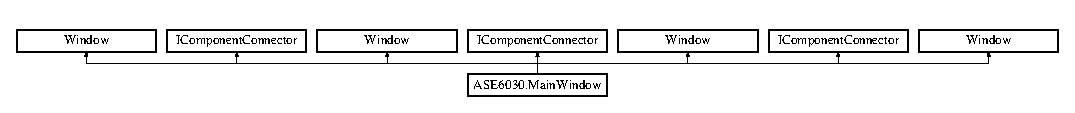
\includegraphics[height=1.073825cm]{class_a_s_e6030_1_1_main_window}
\end{center}
\end{figure}
\subsection*{Public Member Functions}
\begin{DoxyCompactItemize}
\item 
\mbox{\Hypertarget{class_a_s_e6030_1_1_main_window_adeaea371e5e8ae0d36da0488e3f573a9}\label{class_a_s_e6030_1_1_main_window_adeaea371e5e8ae0d36da0488e3f573a9}} 
void {\bfseries update\+Call} (Sorted\+Dictionary$<$ string, dynamic $>$ state)
\item 
\mbox{\Hypertarget{class_a_s_e6030_1_1_main_window_a79b6db853cf517f0df08f041b207e7e6}\label{class_a_s_e6030_1_1_main_window_a79b6db853cf517f0df08f041b207e7e6}} 
void {\bfseries update\+Process\+Flow} (int step)
\item 
void \hyperlink{class_a_s_e6030_1_1_main_window_ae87e50858240332fce20264ac23638e8}{Initialize\+Component} ()
\begin{DoxyCompactList}\small\item\em Initialize\+Component \end{DoxyCompactList}\item 
void \hyperlink{class_a_s_e6030_1_1_main_window_ae87e50858240332fce20264ac23638e8}{Initialize\+Component} ()
\begin{DoxyCompactList}\small\item\em Initialize\+Component \end{DoxyCompactList}\item 
void \hyperlink{class_a_s_e6030_1_1_main_window_ae87e50858240332fce20264ac23638e8}{Initialize\+Component} ()
\begin{DoxyCompactList}\small\item\em Initialize\+Component \end{DoxyCompactList}\end{DoxyCompactItemize}
\subsection*{Private Member Functions}
\begin{DoxyCompactItemize}
\item 
\mbox{\Hypertarget{class_a_s_e6030_1_1_main_window_a3d5fad3a2b1028ab274a65a9beefd608}\label{class_a_s_e6030_1_1_main_window_a3d5fad3a2b1028ab274a65a9beefd608}} 
void {\bfseries set\+Parameters} ()
\item 
\mbox{\Hypertarget{class_a_s_e6030_1_1_main_window_ace6840767bfc4469c5f4571d9605b5f6}\label{class_a_s_e6030_1_1_main_window_ace6840767bfc4469c5f4571d9605b5f6}} 
void {\bfseries Err} (string e)
\item 
\mbox{\Hypertarget{class_a_s_e6030_1_1_main_window_a0fdb876c1210d2f9d5092171da0e96dd}\label{class_a_s_e6030_1_1_main_window_a0fdb876c1210d2f9d5092171da0e96dd}} 
void {\bfseries Start\+Button\+\_\+\+Click} (object sender, Routed\+Event\+Args e)
\item 
\mbox{\Hypertarget{class_a_s_e6030_1_1_main_window_a3f5f58bf9603fa994e7501b10cbf7d97}\label{class_a_s_e6030_1_1_main_window_a3f5f58bf9603fa994e7501b10cbf7d97}} 
void {\bfseries Abort\+Button\+\_\+\+Click} (object sender, Routed\+Event\+Args e)
\item 
\mbox{\Hypertarget{class_a_s_e6030_1_1_main_window_aafd537e91cef65c5f1206de37ec82433}\label{class_a_s_e6030_1_1_main_window_aafd537e91cef65c5f1206de37ec82433}} 
void {\bfseries Connect\+Button\+\_\+\+Click} (object sender, Routed\+Event\+Args e)
\item 
\mbox{\Hypertarget{class_a_s_e6030_1_1_main_window_aedac51ed593438f7c9e834f86310b16d}\label{class_a_s_e6030_1_1_main_window_aedac51ed593438f7c9e834f86310b16d}} 
void {\bfseries Simulator\+Radio\+Button\+\_\+\+Checked} (object sender, Routed\+Event\+Args e)
\item 
\mbox{\Hypertarget{class_a_s_e6030_1_1_main_window_afb968f7e70b4e02f70ed61cdd3b6d12b}\label{class_a_s_e6030_1_1_main_window_afb968f7e70b4e02f70ed61cdd3b6d12b}} 
void {\bfseries update\+State} (Sorted\+Dictionary$<$ string, dynamic $>$ state)
\item 
\mbox{\Hypertarget{class_a_s_e6030_1_1_main_window_a7f00ab98e7c44c2d97e196593aec4e5c}\label{class_a_s_e6030_1_1_main_window_a7f00ab98e7c44c2d97e196593aec4e5c}} 
void {\bfseries update\+View} ()
\item 
\mbox{\Hypertarget{class_a_s_e6030_1_1_main_window_a447cb8531e21b4c80ff7021c6e747a23}\label{class_a_s_e6030_1_1_main_window_a447cb8531e21b4c80ff7021c6e747a23}} 
void {\bfseries update\+Process\+View} (int step)
\item 
\mbox{\Hypertarget{class_a_s_e6030_1_1_main_window_aece2fb1ce86f6eadf27e6baf704e5004}\label{class_a_s_e6030_1_1_main_window_aece2fb1ce86f6eadf27e6baf704e5004}} 
void {\bfseries Device\+Radio\+Button\+\_\+\+Checked} (object sender, Routed\+Event\+Args e)
\item 
\mbox{\Hypertarget{class_a_s_e6030_1_1_main_window_a630c8264730869e95be667655adaa6e7}\label{class_a_s_e6030_1_1_main_window_a630c8264730869e95be667655adaa6e7}} 
void {\bfseries Impregnation\+Input\+\_\+\+Text\+Changed} (object sender, Text\+Changed\+Event\+Args e)
\item 
\mbox{\Hypertarget{class_a_s_e6030_1_1_main_window_acb3d901ff9cac3d38aeb40c2aa3eae85}\label{class_a_s_e6030_1_1_main_window_acb3d901ff9cac3d38aeb40c2aa3eae85}} 
void {\bfseries Cooking\+Time\+Input\+\_\+\+Text\+Changed} (object sender, Text\+Changed\+Event\+Args e)
\item 
\mbox{\Hypertarget{class_a_s_e6030_1_1_main_window_a51d086539ee4b9a50a935a62227152d4}\label{class_a_s_e6030_1_1_main_window_a51d086539ee4b9a50a935a62227152d4}} 
void {\bfseries Cooking\+Pressure\+Input\+\_\+\+Text\+Changed} (object sender, Text\+Changed\+Event\+Args e)
\item 
\mbox{\Hypertarget{class_a_s_e6030_1_1_main_window_aa72c9d337436f936081b639aede4d3a3}\label{class_a_s_e6030_1_1_main_window_aa72c9d337436f936081b639aede4d3a3}} 
void {\bfseries Cooking\+Temperature\+Input\+\_\+\+Text\+Changed} (object sender, Text\+Changed\+Event\+Args e)
\item 
\mbox{\Hypertarget{class_a_s_e6030_1_1_main_window_a093699eefeec90be0b6776cf1cff57ec}\label{class_a_s_e6030_1_1_main_window_a093699eefeec90be0b6776cf1cff57ec}} 
void {\bfseries Gain\+Input\+\_\+\+Text\+Changed} (object sender, Text\+Changed\+Event\+Args e)
\item 
\mbox{\Hypertarget{class_a_s_e6030_1_1_main_window_a2553ee8521aa0a3776706b93fe5bc711}\label{class_a_s_e6030_1_1_main_window_a2553ee8521aa0a3776706b93fe5bc711}} 
void {\bfseries Integration\+Time\+Input\+\_\+\+Text\+Changed} (object sender, Text\+Changed\+Event\+Args e)
\item 
\mbox{\Hypertarget{class_a_s_e6030_1_1_main_window_a5296565cd53cda08d5f39b8903961bee}\label{class_a_s_e6030_1_1_main_window_a5296565cd53cda08d5f39b8903961bee}} 
void System.\+Windows.\+Markup.\+I\+Component\+Connector. {\bfseries Connect} (int connection\+Id, object target)
\item 
\mbox{\Hypertarget{class_a_s_e6030_1_1_main_window_a5296565cd53cda08d5f39b8903961bee}\label{class_a_s_e6030_1_1_main_window_a5296565cd53cda08d5f39b8903961bee}} 
void System.\+Windows.\+Markup.\+I\+Component\+Connector. {\bfseries Connect} (int connection\+Id, object target)
\item 
\mbox{\Hypertarget{class_a_s_e6030_1_1_main_window_a5296565cd53cda08d5f39b8903961bee}\label{class_a_s_e6030_1_1_main_window_a5296565cd53cda08d5f39b8903961bee}} 
void System.\+Windows.\+Markup.\+I\+Component\+Connector. {\bfseries Connect} (int connection\+Id, object target)
\end{DoxyCompactItemize}
\subsection*{Private Attributes}
\begin{DoxyCompactItemize}
\item 
\mbox{\Hypertarget{class_a_s_e6030_1_1_main_window_a2b388122bcbcc462675679d09465f431}\label{class_a_s_e6030_1_1_main_window_a2b388122bcbcc462675679d09465f431}} 
\hyperlink{class_a_s_e6030_1_1_controller}{Controller} {\bfseries controller}
\item 
\mbox{\Hypertarget{class_a_s_e6030_1_1_main_window_a160236952bfdea25ba39ae37d78c81a5}\label{class_a_s_e6030_1_1_main_window_a160236952bfdea25ba39ae37d78c81a5}} 
\hyperlink{class_a_s_e6030_1_1_sequence_parameters}{Sequence\+Parameters} {\bfseries parameters}
\item 
\mbox{\Hypertarget{class_a_s_e6030_1_1_main_window_aa4b5b65983bb7226a44e06e13bcaf274}\label{class_a_s_e6030_1_1_main_window_aa4b5b65983bb7226a44e06e13bcaf274}} 
Sorted\+Dictionary$<$ string, dynamic $>$ {\bfseries state}
\item 
\mbox{\Hypertarget{class_a_s_e6030_1_1_main_window_aeab975c1ce7cb61e9335643b388f6eac}\label{class_a_s_e6030_1_1_main_window_aeab975c1ce7cb61e9335643b388f6eac}} 
Solid\+Color\+Brush {\bfseries G\+R\+E\+EN}
\item 
\mbox{\Hypertarget{class_a_s_e6030_1_1_main_window_a5263c77c02edbe3ee3507eae6976368f}\label{class_a_s_e6030_1_1_main_window_a5263c77c02edbe3ee3507eae6976368f}} 
Solid\+Color\+Brush {\bfseries R\+ED}
\item 
\mbox{\Hypertarget{class_a_s_e6030_1_1_main_window_a89e1033a43d014d2bfea4ea332098698}\label{class_a_s_e6030_1_1_main_window_a89e1033a43d014d2bfea4ea332098698}} 
bool {\bfseries \+\_\+content\+Loaded}
\end{DoxyCompactItemize}


\subsection{Detailed Description}
Interaction logic for Main\+Window.\+xaml 

\hyperlink{class_a_s_e6030_1_1_main_window}{Main\+Window} 

\subsection{Member Function Documentation}
\mbox{\Hypertarget{class_a_s_e6030_1_1_main_window_ae87e50858240332fce20264ac23638e8}\label{class_a_s_e6030_1_1_main_window_ae87e50858240332fce20264ac23638e8}} 
\index{A\+S\+E6030\+::\+Main\+Window@{A\+S\+E6030\+::\+Main\+Window}!Initialize\+Component@{Initialize\+Component}}
\index{Initialize\+Component@{Initialize\+Component}!A\+S\+E6030\+::\+Main\+Window@{A\+S\+E6030\+::\+Main\+Window}}
\subsubsection{\texorpdfstring{Initialize\+Component()}{InitializeComponent()}\hspace{0.1cm}{\footnotesize\ttfamily [1/3]}}
{\footnotesize\ttfamily void A\+S\+E6030.\+Main\+Window.\+Initialize\+Component (\begin{DoxyParamCaption}{ }\end{DoxyParamCaption})\hspace{0.3cm}{\ttfamily [inline]}}



Initialize\+Component 

\mbox{\Hypertarget{class_a_s_e6030_1_1_main_window_ae87e50858240332fce20264ac23638e8}\label{class_a_s_e6030_1_1_main_window_ae87e50858240332fce20264ac23638e8}} 
\index{A\+S\+E6030\+::\+Main\+Window@{A\+S\+E6030\+::\+Main\+Window}!Initialize\+Component@{Initialize\+Component}}
\index{Initialize\+Component@{Initialize\+Component}!A\+S\+E6030\+::\+Main\+Window@{A\+S\+E6030\+::\+Main\+Window}}
\subsubsection{\texorpdfstring{Initialize\+Component()}{InitializeComponent()}\hspace{0.1cm}{\footnotesize\ttfamily [2/3]}}
{\footnotesize\ttfamily void A\+S\+E6030.\+Main\+Window.\+Initialize\+Component (\begin{DoxyParamCaption}{ }\end{DoxyParamCaption})\hspace{0.3cm}{\ttfamily [inline]}}



Initialize\+Component 

\mbox{\Hypertarget{class_a_s_e6030_1_1_main_window_ae87e50858240332fce20264ac23638e8}\label{class_a_s_e6030_1_1_main_window_ae87e50858240332fce20264ac23638e8}} 
\index{A\+S\+E6030\+::\+Main\+Window@{A\+S\+E6030\+::\+Main\+Window}!Initialize\+Component@{Initialize\+Component}}
\index{Initialize\+Component@{Initialize\+Component}!A\+S\+E6030\+::\+Main\+Window@{A\+S\+E6030\+::\+Main\+Window}}
\subsubsection{\texorpdfstring{Initialize\+Component()}{InitializeComponent()}\hspace{0.1cm}{\footnotesize\ttfamily [3/3]}}
{\footnotesize\ttfamily void A\+S\+E6030.\+Main\+Window.\+Initialize\+Component (\begin{DoxyParamCaption}{ }\end{DoxyParamCaption})\hspace{0.3cm}{\ttfamily [inline]}}



Initialize\+Component 



The documentation for this class was generated from the following files\+:\begin{DoxyCompactItemize}
\item 
A\+S\+E6030/Main\+Window.\+xaml.\+cs\item 
A\+S\+E6030/obj/x86/\+Debug/Main\+Window.\+g.\+cs\item 
A\+S\+E6030/obj/x86/\+Debug/Main\+Window.\+g.\+i.\+cs\end{DoxyCompactItemize}

\hypertarget{class_a_s_e6030_1_1_on_off_valve}{}\section{A\+S\+E6030.\+On\+Off\+Valve Class Reference}
\label{class_a_s_e6030_1_1_on_off_valve}\index{A\+S\+E6030.\+On\+Off\+Valve@{A\+S\+E6030.\+On\+Off\+Valve}}
\subsection*{Public Member Functions}
\begin{DoxyCompactItemize}
\item 
\mbox{\Hypertarget{class_a_s_e6030_1_1_on_off_valve_a210880c9d65d53684d468e0290b84772}\label{class_a_s_e6030_1_1_on_off_valve_a210880c9d65d53684d468e0290b84772}} 
{\bfseries On\+Off\+Valve} (String name, ref Tut.\+Mpp\+Opc\+Ua\+Client\+Lib.\+Mpp\+Client client)
\item 
\mbox{\Hypertarget{class_a_s_e6030_1_1_on_off_valve_a682309032082c36a32daa1f7672e4101}\label{class_a_s_e6030_1_1_on_off_valve_a682309032082c36a32daa1f7672e4101}} 
void {\bfseries open} ()
\item 
\mbox{\Hypertarget{class_a_s_e6030_1_1_on_off_valve_a4c878ae2b5970dff941dceb37f0aa863}\label{class_a_s_e6030_1_1_on_off_valve_a4c878ae2b5970dff941dceb37f0aa863}} 
void {\bfseries close} ()
\end{DoxyCompactItemize}


The documentation for this class was generated from the following file\+:\begin{DoxyCompactItemize}
\item 
A\+S\+E6030/On\+Off\+Valve.\+cs\end{DoxyCompactItemize}

\hypertarget{class_a_s_e6030_1_1_pump}{}\section{A\+S\+E6030.\+Pump Class Reference}
\label{class_a_s_e6030_1_1_pump}\index{A\+S\+E6030.\+Pump@{A\+S\+E6030.\+Pump}}


Class for controlling a pump  


\subsection*{Public Member Functions}
\begin{DoxyCompactItemize}
\item 
\hyperlink{class_a_s_e6030_1_1_pump_ac23356a1375f9dc895beeb922721635d}{Pump} (String name, ref Tut.\+Mpp\+Opc\+Ua\+Client\+Lib.\+Mpp\+Client client)
\begin{DoxyCompactList}\small\item\em Constructor \end{DoxyCompactList}\item 
void \hyperlink{class_a_s_e6030_1_1_pump_a80e39e01a6a3fdf187f743991004c4ed}{turn\+On} ()
\begin{DoxyCompactList}\small\item\em Set pump preset and turn on the pump \end{DoxyCompactList}\item 
void \hyperlink{class_a_s_e6030_1_1_pump_aeaca891e7c6220bf12e070c4096c8140}{turn\+Off} ()
\begin{DoxyCompactList}\small\item\em Turn on the pump \end{DoxyCompactList}\item 
void \hyperlink{class_a_s_e6030_1_1_pump_a25c0c51e6e9fbddecdf94f3523b971ad}{set\+Preset} ()
\begin{DoxyCompactList}\small\item\em Set pump preset \end{DoxyCompactList}\end{DoxyCompactItemize}


\subsection{Detailed Description}
Class for controlling a pump 

Creates an object instance of a pump that can be used to control the pump. 

\subsection{Constructor \& Destructor Documentation}
\mbox{\Hypertarget{class_a_s_e6030_1_1_pump_ac23356a1375f9dc895beeb922721635d}\label{class_a_s_e6030_1_1_pump_ac23356a1375f9dc895beeb922721635d}} 
\index{A\+S\+E6030\+::\+Pump@{A\+S\+E6030\+::\+Pump}!Pump@{Pump}}
\index{Pump@{Pump}!A\+S\+E6030\+::\+Pump@{A\+S\+E6030\+::\+Pump}}
\subsubsection{\texorpdfstring{Pump()}{Pump()}}
{\footnotesize\ttfamily A\+S\+E6030.\+Pump.\+Pump (\begin{DoxyParamCaption}\item[{String}]{name,  }\item[{ref Tut.\+Mpp\+Opc\+Ua\+Client\+Lib.\+Mpp\+Client}]{client }\end{DoxyParamCaption})\hspace{0.3cm}{\ttfamily [inline]}}



Constructor 


\begin{DoxyParams}{Parameters}
{\em name} & Name (code) of the corresponding device. Example\+: \char`\"{}\+P100\char`\"{}\\
\hline
{\em client} & Reference to Mpp\+Client object\\
\hline
\end{DoxyParams}


\subsection{Member Function Documentation}
\mbox{\Hypertarget{class_a_s_e6030_1_1_pump_a25c0c51e6e9fbddecdf94f3523b971ad}\label{class_a_s_e6030_1_1_pump_a25c0c51e6e9fbddecdf94f3523b971ad}} 
\index{A\+S\+E6030\+::\+Pump@{A\+S\+E6030\+::\+Pump}!set\+Preset@{set\+Preset}}
\index{set\+Preset@{set\+Preset}!A\+S\+E6030\+::\+Pump@{A\+S\+E6030\+::\+Pump}}
\subsubsection{\texorpdfstring{set\+Preset()}{setPreset()}}
{\footnotesize\ttfamily void A\+S\+E6030.\+Pump.\+set\+Preset (\begin{DoxyParamCaption}{ }\end{DoxyParamCaption})\hspace{0.3cm}{\ttfamily [inline]}}



Set pump preset 

\mbox{\Hypertarget{class_a_s_e6030_1_1_pump_aeaca891e7c6220bf12e070c4096c8140}\label{class_a_s_e6030_1_1_pump_aeaca891e7c6220bf12e070c4096c8140}} 
\index{A\+S\+E6030\+::\+Pump@{A\+S\+E6030\+::\+Pump}!turn\+Off@{turn\+Off}}
\index{turn\+Off@{turn\+Off}!A\+S\+E6030\+::\+Pump@{A\+S\+E6030\+::\+Pump}}
\subsubsection{\texorpdfstring{turn\+Off()}{turnOff()}}
{\footnotesize\ttfamily void A\+S\+E6030.\+Pump.\+turn\+Off (\begin{DoxyParamCaption}{ }\end{DoxyParamCaption})\hspace{0.3cm}{\ttfamily [inline]}}



Turn on the pump 

\mbox{\Hypertarget{class_a_s_e6030_1_1_pump_a80e39e01a6a3fdf187f743991004c4ed}\label{class_a_s_e6030_1_1_pump_a80e39e01a6a3fdf187f743991004c4ed}} 
\index{A\+S\+E6030\+::\+Pump@{A\+S\+E6030\+::\+Pump}!turn\+On@{turn\+On}}
\index{turn\+On@{turn\+On}!A\+S\+E6030\+::\+Pump@{A\+S\+E6030\+::\+Pump}}
\subsubsection{\texorpdfstring{turn\+On()}{turnOn()}}
{\footnotesize\ttfamily void A\+S\+E6030.\+Pump.\+turn\+On (\begin{DoxyParamCaption}{ }\end{DoxyParamCaption})\hspace{0.3cm}{\ttfamily [inline]}}



Set pump preset and turn on the pump 



The documentation for this class was generated from the following file\+:\begin{DoxyCompactItemize}
\item 
A\+S\+E6030/Pump.\+cs\end{DoxyCompactItemize}

\hypertarget{class_a_s_e6030_1_1_sequence_parameters}{}\section{A\+S\+E6030.\+Sequence\+Parameters Class Reference}
\label{class_a_s_e6030_1_1_sequence_parameters}\index{A\+S\+E6030.\+Sequence\+Parameters@{A\+S\+E6030.\+Sequence\+Parameters}}


Class for saving the sequence parameters from user.  


\subsection*{Public Attributes}
\begin{DoxyCompactItemize}
\item 
\mbox{\Hypertarget{class_a_s_e6030_1_1_sequence_parameters_a9f894780c256e1d4ccba4d528689db2d}\label{class_a_s_e6030_1_1_sequence_parameters_a9f894780c256e1d4ccba4d528689db2d}} 
int \hyperlink{class_a_s_e6030_1_1_sequence_parameters_a9f894780c256e1d4ccba4d528689db2d}{impregnation\+Time}
\begin{DoxyCompactList}\small\item\em Impregnation time. \end{DoxyCompactList}\item 
\mbox{\Hypertarget{class_a_s_e6030_1_1_sequence_parameters_a849f7bfb15f35ea4ca038f4c4e5f147c}\label{class_a_s_e6030_1_1_sequence_parameters_a849f7bfb15f35ea4ca038f4c4e5f147c}} 
int \hyperlink{class_a_s_e6030_1_1_sequence_parameters_a849f7bfb15f35ea4ca038f4c4e5f147c}{cooking\+Time}
\begin{DoxyCompactList}\small\item\em Cooking time. \end{DoxyCompactList}\item 
\mbox{\Hypertarget{class_a_s_e6030_1_1_sequence_parameters_aa6ea81d58306fa849f0c15d1f4d2331c}\label{class_a_s_e6030_1_1_sequence_parameters_aa6ea81d58306fa849f0c15d1f4d2331c}} 
double \hyperlink{class_a_s_e6030_1_1_sequence_parameters_aa6ea81d58306fa849f0c15d1f4d2331c}{cooking\+Temperature}
\begin{DoxyCompactList}\small\item\em Cooking temperature. \end{DoxyCompactList}\item 
\mbox{\Hypertarget{class_a_s_e6030_1_1_sequence_parameters_a3541c0320c22637b3566458078f2865d}\label{class_a_s_e6030_1_1_sequence_parameters_a3541c0320c22637b3566458078f2865d}} 
int \hyperlink{class_a_s_e6030_1_1_sequence_parameters_a3541c0320c22637b3566458078f2865d}{cooking\+Pressure}
\begin{DoxyCompactList}\small\item\em Cooking pressure. \end{DoxyCompactList}\item 
\mbox{\Hypertarget{class_a_s_e6030_1_1_sequence_parameters_a54ef8f65093e929f9ba6eee0531502f6}\label{class_a_s_e6030_1_1_sequence_parameters_a54ef8f65093e929f9ba6eee0531502f6}} 
double \hyperlink{class_a_s_e6030_1_1_sequence_parameters_a54ef8f65093e929f9ba6eee0531502f6}{gain}
\begin{DoxyCompactList}\small\item\em PI \hyperlink{class_a_s_e6030_1_1_controller}{Controller} gain. \end{DoxyCompactList}\item 
\mbox{\Hypertarget{class_a_s_e6030_1_1_sequence_parameters_ad949634825a6ec898ea53e5483a6ba50}\label{class_a_s_e6030_1_1_sequence_parameters_ad949634825a6ec898ea53e5483a6ba50}} 
double \hyperlink{class_a_s_e6030_1_1_sequence_parameters_ad949634825a6ec898ea53e5483a6ba50}{integration\+Time}
\begin{DoxyCompactList}\small\item\em PI controller integration time. \end{DoxyCompactList}\end{DoxyCompactItemize}


\subsection{Detailed Description}
Class for saving the sequence parameters from user. 

For now used only as a struct, but could also be used to handle the input type and range check. 

The documentation for this class was generated from the following file\+:\begin{DoxyCompactItemize}
\item 
A\+S\+E6030/Sequence\+Parameters.\+cs\end{DoxyCompactItemize}

\hypertarget{class_controller_unit_test_1_1_unit_test1}{}\section{Controller\+Unit\+Test.\+Unit\+Test1 Class Reference}
\label{class_controller_unit_test_1_1_unit_test1}\index{Controller\+Unit\+Test.\+Unit\+Test1@{Controller\+Unit\+Test.\+Unit\+Test1}}


Unit test for Controller class  


\subsection*{Public Member Functions}
\begin{DoxyCompactItemize}
\item 
void \hyperlink{class_controller_unit_test_1_1_unit_test1_ab5f5063ecc6c61fcddd18f3ef6694868}{Correct\+Values} ()
\begin{DoxyCompactList}\small\item\em Testing for user input of some correct values \end{DoxyCompactList}\item 
void \hyperlink{class_controller_unit_test_1_1_unit_test1_a1191a8c6fa2b4ff8b6293cc5a2680c19}{Max\+Pressure} ()
\begin{DoxyCompactList}\small\item\em Testing for the upper limit of user input for cooking pressure \end{DoxyCompactList}\item 
void \hyperlink{class_controller_unit_test_1_1_unit_test1_a7bdcd66725dc66a60616781b47d4cf11}{Too\+Low\+Temperature} ()
\begin{DoxyCompactList}\small\item\em Testing for too low user input for cooking temperature \end{DoxyCompactList}\item 
void \hyperlink{class_controller_unit_test_1_1_unit_test1_ad6301b75ca38599999e9c20b65731595}{Too\+High\+Temperature} ()
\begin{DoxyCompactList}\small\item\em Testing for too high user input for cooking temperature \end{DoxyCompactList}\item 
void \hyperlink{class_controller_unit_test_1_1_unit_test1_a489508b562944eaddd888034be0b66dc}{Too\+High\+Pressure} ()
\begin{DoxyCompactList}\small\item\em Testing for too high user input for cooking pressure \end{DoxyCompactList}\item 
void \hyperlink{class_controller_unit_test_1_1_unit_test1_a83cb8833e8eba5a8ca87257234602e6e}{Too\+Low\+Pressure} ()
\begin{DoxyCompactList}\small\item\em Testing for too low user input for cooking pressure \end{DoxyCompactList}\item 
void \hyperlink{class_controller_unit_test_1_1_unit_test1_a6b88d429df0c18261c8487cd785230b5}{Legal\+Inputs} ()
\begin{DoxyCompactList}\small\item\em Testing for legal user inputs. Type double inputs with 0.\+01 accuracy \end{DoxyCompactList}\item 
void \hyperlink{class_controller_unit_test_1_1_unit_test1_abc3e4821a5f8e5b0555298e835fec144}{U\+R\+L\+Test} ()
\begin{DoxyCompactList}\small\item\em Test for using random string as U\+RL. Should use simulator as default \end{DoxyCompactList}\end{DoxyCompactItemize}


\subsection{Detailed Description}
Unit test for Controller class 



\subsection{Member Function Documentation}
\mbox{\Hypertarget{class_controller_unit_test_1_1_unit_test1_ab5f5063ecc6c61fcddd18f3ef6694868}\label{class_controller_unit_test_1_1_unit_test1_ab5f5063ecc6c61fcddd18f3ef6694868}} 
\index{Controller\+Unit\+Test\+::\+Unit\+Test1@{Controller\+Unit\+Test\+::\+Unit\+Test1}!Correct\+Values@{Correct\+Values}}
\index{Correct\+Values@{Correct\+Values}!Controller\+Unit\+Test\+::\+Unit\+Test1@{Controller\+Unit\+Test\+::\+Unit\+Test1}}
\subsubsection{\texorpdfstring{Correct\+Values()}{CorrectValues()}}
{\footnotesize\ttfamily void Controller\+Unit\+Test.\+Unit\+Test1.\+Correct\+Values (\begin{DoxyParamCaption}{ }\end{DoxyParamCaption})\hspace{0.3cm}{\ttfamily [inline]}}



Testing for user input of some correct values 

\mbox{\Hypertarget{class_controller_unit_test_1_1_unit_test1_a6b88d429df0c18261c8487cd785230b5}\label{class_controller_unit_test_1_1_unit_test1_a6b88d429df0c18261c8487cd785230b5}} 
\index{Controller\+Unit\+Test\+::\+Unit\+Test1@{Controller\+Unit\+Test\+::\+Unit\+Test1}!Legal\+Inputs@{Legal\+Inputs}}
\index{Legal\+Inputs@{Legal\+Inputs}!Controller\+Unit\+Test\+::\+Unit\+Test1@{Controller\+Unit\+Test\+::\+Unit\+Test1}}
\subsubsection{\texorpdfstring{Legal\+Inputs()}{LegalInputs()}}
{\footnotesize\ttfamily void Controller\+Unit\+Test.\+Unit\+Test1.\+Legal\+Inputs (\begin{DoxyParamCaption}{ }\end{DoxyParamCaption})\hspace{0.3cm}{\ttfamily [inline]}}



Testing for legal user inputs. Type double inputs with 0.\+01 accuracy 

Test for legal int inputs

Test for cooking temperature inputs \mbox{\Hypertarget{class_controller_unit_test_1_1_unit_test1_a1191a8c6fa2b4ff8b6293cc5a2680c19}\label{class_controller_unit_test_1_1_unit_test1_a1191a8c6fa2b4ff8b6293cc5a2680c19}} 
\index{Controller\+Unit\+Test\+::\+Unit\+Test1@{Controller\+Unit\+Test\+::\+Unit\+Test1}!Max\+Pressure@{Max\+Pressure}}
\index{Max\+Pressure@{Max\+Pressure}!Controller\+Unit\+Test\+::\+Unit\+Test1@{Controller\+Unit\+Test\+::\+Unit\+Test1}}
\subsubsection{\texorpdfstring{Max\+Pressure()}{MaxPressure()}}
{\footnotesize\ttfamily void Controller\+Unit\+Test.\+Unit\+Test1.\+Max\+Pressure (\begin{DoxyParamCaption}{ }\end{DoxyParamCaption})\hspace{0.3cm}{\ttfamily [inline]}}



Testing for the upper limit of user input for cooking pressure 

\mbox{\Hypertarget{class_controller_unit_test_1_1_unit_test1_a489508b562944eaddd888034be0b66dc}\label{class_controller_unit_test_1_1_unit_test1_a489508b562944eaddd888034be0b66dc}} 
\index{Controller\+Unit\+Test\+::\+Unit\+Test1@{Controller\+Unit\+Test\+::\+Unit\+Test1}!Too\+High\+Pressure@{Too\+High\+Pressure}}
\index{Too\+High\+Pressure@{Too\+High\+Pressure}!Controller\+Unit\+Test\+::\+Unit\+Test1@{Controller\+Unit\+Test\+::\+Unit\+Test1}}
\subsubsection{\texorpdfstring{Too\+High\+Pressure()}{TooHighPressure()}}
{\footnotesize\ttfamily void Controller\+Unit\+Test.\+Unit\+Test1.\+Too\+High\+Pressure (\begin{DoxyParamCaption}{ }\end{DoxyParamCaption})\hspace{0.3cm}{\ttfamily [inline]}}



Testing for too high user input for cooking pressure 

\mbox{\Hypertarget{class_controller_unit_test_1_1_unit_test1_ad6301b75ca38599999e9c20b65731595}\label{class_controller_unit_test_1_1_unit_test1_ad6301b75ca38599999e9c20b65731595}} 
\index{Controller\+Unit\+Test\+::\+Unit\+Test1@{Controller\+Unit\+Test\+::\+Unit\+Test1}!Too\+High\+Temperature@{Too\+High\+Temperature}}
\index{Too\+High\+Temperature@{Too\+High\+Temperature}!Controller\+Unit\+Test\+::\+Unit\+Test1@{Controller\+Unit\+Test\+::\+Unit\+Test1}}
\subsubsection{\texorpdfstring{Too\+High\+Temperature()}{TooHighTemperature()}}
{\footnotesize\ttfamily void Controller\+Unit\+Test.\+Unit\+Test1.\+Too\+High\+Temperature (\begin{DoxyParamCaption}{ }\end{DoxyParamCaption})\hspace{0.3cm}{\ttfamily [inline]}}



Testing for too high user input for cooking temperature 

\mbox{\Hypertarget{class_controller_unit_test_1_1_unit_test1_a83cb8833e8eba5a8ca87257234602e6e}\label{class_controller_unit_test_1_1_unit_test1_a83cb8833e8eba5a8ca87257234602e6e}} 
\index{Controller\+Unit\+Test\+::\+Unit\+Test1@{Controller\+Unit\+Test\+::\+Unit\+Test1}!Too\+Low\+Pressure@{Too\+Low\+Pressure}}
\index{Too\+Low\+Pressure@{Too\+Low\+Pressure}!Controller\+Unit\+Test\+::\+Unit\+Test1@{Controller\+Unit\+Test\+::\+Unit\+Test1}}
\subsubsection{\texorpdfstring{Too\+Low\+Pressure()}{TooLowPressure()}}
{\footnotesize\ttfamily void Controller\+Unit\+Test.\+Unit\+Test1.\+Too\+Low\+Pressure (\begin{DoxyParamCaption}{ }\end{DoxyParamCaption})\hspace{0.3cm}{\ttfamily [inline]}}



Testing for too low user input for cooking pressure 

\mbox{\Hypertarget{class_controller_unit_test_1_1_unit_test1_a7bdcd66725dc66a60616781b47d4cf11}\label{class_controller_unit_test_1_1_unit_test1_a7bdcd66725dc66a60616781b47d4cf11}} 
\index{Controller\+Unit\+Test\+::\+Unit\+Test1@{Controller\+Unit\+Test\+::\+Unit\+Test1}!Too\+Low\+Temperature@{Too\+Low\+Temperature}}
\index{Too\+Low\+Temperature@{Too\+Low\+Temperature}!Controller\+Unit\+Test\+::\+Unit\+Test1@{Controller\+Unit\+Test\+::\+Unit\+Test1}}
\subsubsection{\texorpdfstring{Too\+Low\+Temperature()}{TooLowTemperature()}}
{\footnotesize\ttfamily void Controller\+Unit\+Test.\+Unit\+Test1.\+Too\+Low\+Temperature (\begin{DoxyParamCaption}{ }\end{DoxyParamCaption})\hspace{0.3cm}{\ttfamily [inline]}}



Testing for too low user input for cooking temperature 

\mbox{\Hypertarget{class_controller_unit_test_1_1_unit_test1_abc3e4821a5f8e5b0555298e835fec144}\label{class_controller_unit_test_1_1_unit_test1_abc3e4821a5f8e5b0555298e835fec144}} 
\index{Controller\+Unit\+Test\+::\+Unit\+Test1@{Controller\+Unit\+Test\+::\+Unit\+Test1}!U\+R\+L\+Test@{U\+R\+L\+Test}}
\index{U\+R\+L\+Test@{U\+R\+L\+Test}!Controller\+Unit\+Test\+::\+Unit\+Test1@{Controller\+Unit\+Test\+::\+Unit\+Test1}}
\subsubsection{\texorpdfstring{U\+R\+L\+Test()}{URLTest()}}
{\footnotesize\ttfamily void Controller\+Unit\+Test.\+Unit\+Test1.\+U\+R\+L\+Test (\begin{DoxyParamCaption}{ }\end{DoxyParamCaption})\hspace{0.3cm}{\ttfamily [inline]}}



Test for using random string as U\+RL. Should use simulator as default 



The documentation for this class was generated from the following file\+:\begin{DoxyCompactItemize}
\item 
A\+S\+E6030\+Unit\+Test/Unit\+Test1.\+cs\end{DoxyCompactItemize}

%--- End generated contents ---

% Index
\backmatter
\newpage
\phantomsection
\clearemptydoublepage
\addcontentsline{toc}{chapter}{Index}
\printindex

\end{document}
